\chapter{分离变量法}

% 本章依次讨论直角坐标系、柱坐标系、球坐标系中的分离变量法.

分离变量法的基本思想是, 
先求出具有变量分离形式且满足边界条件的特解,
然后根据叠加原理作出这些解的线性叠加, 
最后由其余的定解条件确定待定系数,得到定解问题的解.
分离变量法的特点是把偏微分方程化为常微分方程来处理,使问题化难为简.

分离变量法的关键步骤是求解本征值问题, 
即求解含有参量 $\lambda$ 的齐次常微分方程的边值问题. 
其边界条件分别为齐次边界条件、周期性边界条件和自然边界条件
(有界性边界条件).


% 接着,我们介绍施图姆-刘维尔本征值问题, 
% 它是分离变量法的理论基础. 
% 通过这一节的讨论,让我们从新的理论高度认识分离变量法.

% 分离变量法适用于波动问题、
% 输运问题和稳定场问题在特殊域(矩形、长方形、圆、圆球、圆柱体等) 
% 中的定解问题, 因为这些特殊域正好常常在实际问题中出现,
% 这是分离变量法有广泛的应用的原因.

% \section{直角坐标系下的分离变量法}
\label{sec:cartesian}


本节先讨论齐次方程及齐次边界条件的定解问题, 随后讨论对非齐次方程及非齐次边界条件的处理,最后讨论高维的情形.

\subsection{齐次方程及齐次边界条件的定解问题}
首先通过实例说明用分离变量法解题的六个基本步骤.

% \begin{examplebox}{求两端固定的弦自由振动的规律.}

求两端固定的弦自由振动的规律.
定解问题为
\begin{equation}
    \begin{cases}u_{t t}-a^{2} u_{x x}=0, & 0<x<l, \quad t>0 
        \\ u(0, t)=0, \quad u(l, t)=0 & 
        \\ u(x, 0)=\varphi(x), \quad u_{t}(x, 0)=\psi(x) & 
    \end{cases}
    \label{eq:string_vibration_equation}
\end{equation}

\begin{enumerate}
  \item \textbf{分离变量}

    令
    \begin{equation}
        u(x, t)=X(x) T(t)
        \label{eq:uxt}
    \end{equation}
    将式\eqref{eq:uxt}代人泛定方程\eqref{eq:string_vibration_equation}, 可得
    $$
    X(x) T^{\prime \prime}(t)-a^{2} X^{\prime \prime}(x) T(t)=0
    $$
即
$$
\frac{X^{\prime \prime}(x)}{X(x)}=\frac{T^{\prime \prime}(t)}{a^{2} T(t)}
$$

由于上式右端与 $x$ 无关,左端与 $t$ 无关, 而 $x$ 与 $t$ 又是互相独立的变量, 
因此上式只有等于常数才能成立. 令常数为 $-\lambda$, 便得到两个常微分方程
\begin{equation}
    \begin{aligned}
        & X^{\prime \prime}(x)+\lambda X(x)=0 \\
        & T^{\prime \prime}(t)+\lambda a^{2} T(t)=0
        \end{aligned}
        \label{eq:XT}
\end{equation}

将式\eqref{eq:uxt}代人边界条件, 可得
$$
u(0, t)=X(0) T(t)=0, \quad u(l, t)=X(l) T(t)=0
$$
若 $T(t)=0$, 代人式 \eqref{eq:uxt} 得 $u(x, t)=0$, 是平庸解, 应略去. 由此得边界条件
\begin{equation}
    X(0)=0, \quad X(l)=0
    \label{eq:boundary}
\end{equation}

\item \textbf{求解本征值问题}

式\eqref{eq:XT}及式\eqref{eq:boundary}构成了常微分方程的边值问题
$$
\left\{\begin{array}{l}
X^{\prime \prime}(x)+\lambda X(x)=0 \\
X(0)=0, \quad X(l)=0
\end{array}\right.
$$
这称为本征值问题. 
可以证明, 只有当 $\lambda$ 取某些特定值时才有非零解,
求解本征值问题就是求解本征值 $\lambda$ 与本征函数 $X(x)$.

现将 $\lambda$ 的取值分三种情况讨论:

\begin{itemize}
    \item 若 $\lambda<0$, 这时方程的通解为 $X(x)=A e^{\sqrt{-\lambda} x}+B e^{-\sqrt{-\lambda} x}$.

        由边界条件 $X(0)=X(l)=0$, 可得
        
        $$
        \left\{\begin{array}{l}
        A+B=0 \\
        A e^{\sqrt{-\lambda l}}+B e^{-\sqrt{-\lambda l}}=0
        \end{array}\right.
        $$
        
        这是关于 $A 、 B$ 的线性齐次方程组, 由于系数行列式不为零, 故 $A=B=0$. 因此 $\lambda<0$ 时, $X(x)$ 无非零解.

    \item 若 $\lambda=0$, 这时方程成为 $X^{\prime \prime}(x)=0$, 它的通解为 $X(x)=A x+B$.

        由边界条件 $X(0)=X(l)=0$ 得 $A=B=0, X(x)$ 也无非零解.
    
    \item 若 $\lambda>0$, 方程的通解为 $X(x)=A \cos \sqrt{\lambda} x+B \sin \sqrt{\lambda} x$.

        由边界条件 $X(0)=0$, 得 $A=0$. 由 $X(l)=0$ 得 $B \sin \sqrt{\lambda} l=0$. 非零解要求 $B \neq 0$, 故
        
        $$
        \sin \sqrt{\lambda} l=0 \quad \text { 即 } \sqrt{\lambda}=\frac{n \pi}{l}, \quad n=1,2, \cdots
        $$
        
        因此本征值 (加上脚标 $n$ ) 及相应的本征函数分别为
        
        $$
        \lambda_{n}=\left(\frac{n \pi}{l}\right)^{2}, \quad n=1,2, \cdots
        $$
        
        $$
        X_{n}(x)=B_{n} \sin \frac{n \pi x}{l}, \quad n=1,2, \cdots
        $$
\end{itemize}





  \item \textbf{求解 $T(t)$ 的常微分方程}
  
    将本征值 $\lambda_{n}=\left(\frac{n \pi}{l}\right)^{2}$ 代入式\eqref{eq:XT}, 得到

    $$
    T^{\prime \prime}(t)+\left(\frac{n \pi a}{l}\right)^{2} T(t)=0
    $$

    它的通解为
    $$
    T_{n}(t)=C_{n} \cos \frac{n \pi a t}{l}+D_{n} \sin \frac{n \pi a t}{l}
    $$
    式中 $C_{n}$ 和 $D_{n}$ 为任意常数.
    
    \item \textbf{作特解的线性叠加}
    
    满足方程及边界条件 \eqref{eq:string_vibration_equation}的一系列特解为
    \begin{equation}
        u_{n}(x, t)=X_{n}(x) T_{n}(t)=\left(C_{n} \cos \frac{n \pi a t}{l}+D_{n} \sin \frac{n \pi a t}{l}\right) \sin \frac{n \pi x}{l}, 
        \label{eq:special_solution}
    \end{equation}
    这里已将任意常数 $B_{n}$ 吸收到任意常数 $C_{n}$ 及 $D_{n}$ 中去了.
    
    特解\eqref{eq:special_solution}一般不满足初始条件, 实际上由式\eqref{eq:special_solution}可得 
    $$
    \begin{aligned}
    u_{n}(x, 0) & =C_{n} \sin \frac{n \pi x}{l} \\
    \left.\frac{\partial u_{n}(x, t)}{\partial t}\right|_{t=0} & =D_{n} \frac{n \pi a}{l} \sin \frac{n \pi x}{l}
    \end{aligned}
    $$

    这表明, 除非 $\varphi(x)$ 和 $\psi(x)$ 同时为 $\sin \frac{n \pi x}{l}$ 的倍数,
     否则任何一个特解不可能满足题目给定的初始条件. 
     但考虑到方程  及边界条件\eqref{eq:string_vibration_equation}都是齐次线性的, 
     因此将所有的特解线性叠加起来, 如果级数收玫, $u(x, t)$ 仍然满足方程 与边界条件. 由此得
    \begin{equation}
        u(x, t)=\sum_{n=1}^{\infty} u_{n}(x, t)=
        \sum_{n=1}^{\infty}\left(C_{n} \cos \frac{n \pi a t}{l}+
        D_{n} \sin \frac{n \pi a t}{l}\right) \sin \frac{n \pi x}{l}
        \label{eq:general_solution}
    \end{equation}
    而待定系数 $C_{n}$ 和 $D_{n}$ 可由初始条件来确定.
    

    \item \textbf{由初始条件确定系数} 
    
        将式\eqref{eq:general_solution}代人初始条件, 即有
        $$
        \begin{gathered}
        \varphi(x)=u(x, 0)=\sum_{n=1}^{\infty} C_{n} \sin \frac{n \pi x}{l} \\
        \psi(x)=u_{t}(x, 0)=\sum_{n=1}^{\infty} D_{n} \frac{n \pi a}{l} \sin \frac{n \pi x}{l}
        \end{gathered}
        $$
        最终系数可由前面傅里叶级数展开来确定系数$C_{n}$ 及 $D_{n}$, 即得定解问题的解.
        $$
        \begin{aligned}
        & C_{n}=\frac{2}{l} \int_{0}^{l} \varphi(x) \sin \frac{n \pi x}{l} d x, \quad n=1,2, \cdots \\
        & D_{n}=\frac{2}{n \pi a} \int_{0}^{l} \psi(x) \sin \frac{n \pi x}{l} d x, \quad n=1,2, \cdots
        \end{aligned}
        $$


        \item \textbf{解的物理意义}
        
        先看级数\eqref{eq:general_solution}的每一项 (即每一个特解)的物理意义.

        \begin{equation}
            u_{n}(x, t)=\left(C_{n} \cos \frac{n \pi a t}{l}+D_{n} \sin \frac{n \pi a t}{l}\right) \sin \frac{n \pi x}{l}
            =E_{n} \cos \left(\omega_{n} t-\varphi_{n}\right) \sin \frac{n \pi x}{l}
            \label{eq:solution_2}
        \end{equation}    
        式中
        $$
        E_{n}=\sqrt{C_{n}^{2}+D_{n}^{2}}, 
            \quad \omega_{n}=\frac{n \pi a}{l}, 
            \quad \varphi_{n}=\tan ^{-1} \frac{D_{n}}{C_{n}}
        $$
        
        如果弦按式\eqref{eq:solution_2}的规律运动时, 
        $x=0$ 及 $x=l$ 这两个端点保持不动. 
        而弦上各点则在各自的平衡位置附近作简谐振动, 
        其振幅分别为 $E_{n}\left|\sin \frac{n \pi x}{l}\right|$. 
        弦的这种形式的运动称为驻波. 
        在点 $x=\frac{m l}{n}(m=0,1, \cdots, n)$ 处, 振幅为零. 
        这些点在整个振动过程中始终保持不动, 称为\textbf{驻波} $u_{n}(x, t)$ 的\textbf{波节}. 
        在点 $x=\frac{2 m+1}{2 n} l(m=0,1$, $\cdots, n-1)$ 处, 
        $\sin \frac{n \pi x}{l}= \pm 1$, 这些点的振幅最大,称为驻波的\textbf{波腹}.
         驻波的\textbf{角频率} $\omega_{n}=\frac{n \pi}{l}$, 
         其中 $n=1$ 的项 $u_{1}(x, t)$ 称为\textbf{基波}, 
         而 $n>1$ 的项 $u_{n}(x, t)$ 称为 \textbf{$n$ 次谐波}, 
         这些驻波也称为两端固定弦的本征振动. 
         因此, 有界弦的任意振动可看作一系列本征振动的叠加.
        
\end{enumerate}





\subsection{非齐次方程及齐次边界条件的定解问题}

% 上一节研究了齐次方程的定解问题. 本节要研究非齐次振动方程和输运方程的定解问题.

% 我们仍然限于齐次的边界条件, 关于非齐次边界条件的处理请看下一节.

本节先介绍傅里叶级数法, 它直接求解非齐次方程的定解问题. 
接着是冲量定理法, 它把非齐次方程的定解问题转化为齐次方程的定解问题然后求解.

\section{(一) 傅里叶级数法}
$\S 8.1$ 中求解两端固定的弦的齐次振动方程定解问题, 得到的解 (8.1.14)具有傅里叶正弦级数的形式, 而且其系数 $A_{n}$ 和 $B_{n}$ 决定于初始条件 $\varphi(x)$ 和 $\psi(x)$ 的傅里叶正弦级数 (8.1.15). 至于采取正弦级数而不是一般的傅里叶级数的形式,则完全是由于两端都是第一类齐次边界条件 $\left.u\right|_{x=0}=0$ 和 $\left.u\right|_{x=l}=0$的原因.

分离变数法得出的这些结果给出提示: 不妨把所求的解本身展开为傅里叶级数, 即

$$
u(x, t)=\sum_{n} T_{n}(t) X_{n}(x)
$$

傅里叶级数 (8.2.1) 的基本函数族 $X_{n}(x)$ 为该定解问题齐次方程在所给齐次边界条件下的本征函数.

由于解是自变数 $x$ 和 $t$ 的函数, 因而 $u(x, t)$ 的傅里叶系数不是常数, 而是时间 $t$ 的函数, 把它记作 $T_{n}(t)$. 将待定解 (8.2.1) 代人泛定方程, 尝试分离出 $T_{n}(t)$ 的常微分方程, 然后求解.

例 1 求解定解问题

$$
\begin{gathered}
u_{t t}-a^{2} u_{x x}=A \cos \frac{\pi x}{l} \sin \omega t ; \\
\left.u_{x}\right|_{x=0}=0,\left.u_{x}\right|_{x=l}=0 ; \\
\left.u\right|_{t=0}=\varphi(x),\left.u_{t}\right|_{t=0}=\psi(x),(0<x<l) .
\end{gathered}
$$

解 级数展开的基本函数应是相应的齐次泛定方程 $u_{t u}-a^{2} u_{x x}=0$ 在所给齐次边界条件 $\left.u_{x}\right|_{x=0}=0$ 和 $\left.u_{x}\right|_{x=l}=0$ 下的本征函数. 我们已经熟悉这些本征函数, 它们是 $\cos \frac{n \pi x}{l}(n=0,1,2, \cdots)$. 这样, 试把所求的解展开为傅里叶余弦级数

$$
u(x, t)=\sum_{n=0}^{\infty} T_{n}(t) \cos \frac{n \pi x}{l}
$$

为了求解 $T_{n}(t)$ ,尝试把这个级数代人非齐次泛定方程 (8.2.2),

$$
\sum_{n=0}^{\infty}\left[T_{n}^{\prime \prime}+\frac{n^{2} \pi^{2} a^{2}}{l^{2}} T_{n}\right] \cos \frac{n \pi x}{l}=A \cos \frac{\pi x}{l} \sin \omega t
$$

等式左边是傅里叶余弦级数, 这提示我们把等式右边也展开为傅里叶余弦级数. 其实, 右边已经是傅里叶余弦级数, 它只有一个单项即 $n=1$ 的项. 于是, 比较两边的系数, 分离出 $T_{n}(t)$ 的常微分方程

$$
T_{1}^{\prime \prime}+\frac{\pi^{2} a^{2}}{l^{2}} T_{1}=A \sin \omega t, \quad T_{n}^{\prime \prime}+\frac{n^{2} \pi^{2} a^{2}}{l^{2}} T_{n}=0, \quad n \neq 1
$$

又把 $u(x, t)$ 的傅里叶余弦级数代人初始条件, 得

$$
\begin{aligned}
& \sum_{n=0}^{\infty} T_{n}(0) \cos \frac{n \pi}{l} x=\varphi(x)=\sum_{n=0}^{\infty} \varphi_{n} \cos \frac{n \pi}{l} x \\
& \sum_{n=0}^{\infty} T_{n}^{\prime}(0) \cos \frac{n \pi}{l} x=\psi(x)=\sum_{n=0}^{\infty} \psi_{n} \cos \frac{n \pi}{l} x .
\end{aligned}
$$

其中 $\varphi_{n} 、 \psi_{n}$ 分别为 $\varphi(x)$ 和 $\psi(x)$ 的傅里叶余弦级数 [ 以 $\cos (n \pi x / l)$ 为基本函数族] 的第 $n$ 个傅里叶系数. 等式 (8.2.5)、(8.2.6) 两边都是傅里叶余弦级数. 由于基本函数族 $\cos (n \pi x / l)$ 的正交性,等式两边对应同一基本函数的傅里叶系数必然相等; 于是得 $T_{n}(t)$ 的非零值初始条件

$$
\begin{aligned}
& \left\{\begin{array}{l}
T_{0}(0)=\varphi_{0}=\frac{1}{l} \int_{0}^{l} \varphi(\xi) d \xi, \\
T_{0}^{\prime}(0)=\psi_{0}=\frac{1}{l} \int_{0}^{l} \psi(\xi) d \xi ;
\end{array}\right. \\
& \left\{\begin{array}{l}
T_{n}(0)=\varphi_{n}=\frac{2}{l} \int_{0}^{l} \varphi(\xi) \cos \frac{n \pi \xi}{l} d \xi, \\
T_{n}^{\prime}(0)=\psi_{n}=\frac{2}{l} \int_{0}^{l} \psi(\xi) \cos \frac{n \pi \xi}{l} d \xi,
\end{array}\right.
\end{aligned}
$$

$T_{n}(t)$ 的常微分方程在初始条件 (8.2.7) 下的解是

$$
\begin{aligned}
& T_{0}(t)=\varphi_{0}+\psi_{0} t \\
& T_{1}(t)=\frac{A l}{\pi a} \frac{1}{\omega^{2}-\pi^{2} a^{2} / l^{2}}\left(\omega \sin \frac{\pi a t}{l}-\frac{\pi a}{l} \sin \omega t\right) \\
&+\varphi_{1} \cos \frac{\pi a t}{l}+\frac{l}{\pi a} \psi_{1} \sin \frac{\pi a t}{l}, \\
& T_{n}(t)=\varphi_{n} \cos ^{*} \frac{n \pi a t}{l}+\frac{l}{n \pi a} \psi_{n} \sin \frac{n \pi a t}{l} \quad(n \neq 0,1)
\end{aligned}
$$

(8.2.9) 的第一项为 $T_{1}(t)$ 的非齐次常微分方程的特解, 满足零值初始条件. (8.2.9) 的后两项之和及 $(8.2 .10)$ 分别为 $T_{1}(t)$ 和 $T_{n}(t)(n \neq 0,1)$ 的齐次
常微分方程的解, 满足非零值初始条件 (8.2.7).

这样, 所求的解是

$$
\begin{aligned}
u(x, t)= & \frac{A l}{\pi a} \cdot \frac{1}{\omega^{2}-\pi^{2} a^{2} / l^{2}}\left(\omega \sin \frac{\pi a t}{l}-\frac{\pi a}{l} \sin \omega t\right) \cos \frac{\pi x}{l}+\varphi_{0}+ \\
& \psi_{0} t+\sum_{n=1}^{\infty}\left(\varphi_{n} \cos \frac{n \pi a t}{l}+\frac{l}{n \pi a} \psi_{n} \sin \frac{n \pi a t}{l}\right) \cos \frac{n \pi x}{l}
\end{aligned}
$$

尝试成功了, 这个方法叫做傅里叶级数法. 很明显, 这个方法的关键在于分离出 $T_{n}(t)$ 的常微分方程, 其中不可混杂着另一自变数 $x$, 这是怎样做到的呢? 原来, 这个级数展开的基本函数 $\cos (n \pi x / l)$ 正是相应齐次方程、齐次边界条件下用分离变数法求得的本征函数, 这才得以分离出 $T_{n}(t)$ 的常微分方程. 因此, 傅里叶级数法一定要与分离变数法相结合才能应用.

齐次振动方程和齐次输运方程问题当然也可以用傅里叶级数法 (结合分离变数法) 求解, 这时得到的 $T_{n}(t)$ 的常微分方程为齐次方程, 求解更容易. 建议读者用这样的方法重新求解上节的定解问题 (8.1.1) (8.1.3) 以及例 1 和例 2 , 这里就不赘述了.

综上所述, 可以看出, 对于振动和输运问题, 不论齐次还是非齐次方程定解问题, 傅里叶级数法结合分离变数法均可应用. 如仅用分离变数法, 则只能用于齐次方程齐次边界条件定解问题.

\section{(二) 冲量定理法}
求解非齐次振动方程和输运方程定解问题还可用冲量定理法. 这里仍然考虑边界条件是齐次的. 应用冲量定理法有一个前提, 即初始条件均取零值. 这其实无损于一般性. 现以两端固定弦的受迫振动为例, 如果初始条件是非零值, 则定解问题为

$$
\begin{aligned}
& u_{t t}-a^{2} u_{x x}=f(x, t) \\
& \left.u\right|_{x=0}=0,\left.u\right|_{x=l}=0 \\
& \left.u\right|_{t=0}=\varphi(x),\left.u_{t}\right|_{t=0}=\psi(x)
\end{aligned}
$$

由于泛定方程和定解条件都是线性的, 可以利用叠加原理, 把 $u$ 分解为 $u^{\mathrm{I}}$ 与 $u^{\mathrm{I}}$ 之和, 即

$$
u(x, t)=u^{\mathrm{I}}(x, t)+u^{\mathrm{I}}(x, t)
$$

并令 $u^{\mathrm{I}} 、 u^{\mathbb{1}}$ 分别满足

$$
\begin{array}{l|l}
u_{t t}^{\mathrm{I}}-a^{2} u_{x x}^{\mathrm{I}}=0, & u_{t t}^{\mathrm{II}}-a^{2} u_{x x}^{\mathrm{I}}=f(x, t), \\
\left.u^{\mathrm{I}}\right|_{x=0}=0,\left.u^{\mathrm{I}}\right|_{x=l}=0, & \left.u^{\mathrm{I}}\right|_{x=0}=0,\left.u^{\mathrm{II}}\right|_{x=l}=0, \\
\left.u^{\mathrm{I}}\right|_{t=0}=\varphi(x),\left.u_{t}^{\mathrm{I}}\right|_{t=0}=\psi(x) . & \left.u^{\mathrm{I}}\right|_{t=0}=0,\left.u_{t}^{\mathbb{I}}\right|_{t=0}=0
\end{array}
$$

把竖线两边对应的式子相叠加, 正好是原来的定解问题. 这样, 问题转化
为求解 $u^{\mathrm{I}}$ 和 $u^{\mathrm{I}} . u^{\mathrm{I}}$ 的初始条件是非零值, 但方程是齐次的, 可用上节方法求解; $u^{\text {II }}$ 的方程是非齐次的, 但初始条件已化为零值, 符合冲量定理法所提出的要求.

现在用冲量定理法来研究弦的非齐次振动方程定解问题

$$
\begin{gathered}
u_{u}-a^{2} u_{x x}=f(x, t) \\
\left.u\right|_{x=0}=0,\left.u\right|_{x=l}=0 \\
\left.u\right|_{t=0}=0,\left.\quad u_{t}\right|_{t=0}=0
\end{gathered}
$$

\section{(1)冲量定量法的物理思想}
首先, 在物理上, 非齐次泛定方程 (8.2.12) 表明, 作用在每单位长弦上的外力 $F(x, t)=\rho f(x, t)$. 它从时刻零持续作用到时刻 $t$, 我们求解的是 $F(x$, $t$ )作用下, 在时刻 $t$ 的各处位移 $u(x, t)$.

冲量定理法的基本物理思想是把持续作用力看成许许多多前后相继的 “瞬时” 力, 把持续作用力引起的振动看作所有 “瞬时” 力引起的振动的叠加. 根据 (5.3.9), 持续作用的力 $F(x, t)$ 可以表示成

$$
\begin{aligned}
F(x, t) & =\int_{0}^{t} F(x, \tau) \delta(t-\tau) d \tau=\rho f(x, t) \\
& =\int_{0}^{t} \rho f(x, \tau) \delta(t-\tau) d \tau,
\end{aligned}
$$

其中 $F(x, \tau) \delta(t-\tau) d \tau$ 为作用在很短的时间区间 $(\tau, \tau+d \tau)$ 上而冲量为 $F(x, \tau) d \tau$ 的 “瞬时” 力. 把该瞬时力引起的振动记为 $u^{(\tau)}(x, t)$, 则 $u^{(\tau)}(x, t)$的定解问题为

$$
\begin{gathered}
u_{t u}^{(\tau)}-a^{2} u_{x x}^{(\tau)}=\frac{F(x, \tau)}{\rho} \delta(t-\tau) d \tau=f(x, \tau) \delta(t-\tau) d \tau \\
\left.u^{(\tau)}\right|_{x=0}=0,\left.u^{(\tau)}\right|_{x=l}=0, \\
\left.u^{(\tau)}\right|_{t=0}=0,\left.u_{t}^{(\tau)}\right|_{t=0}=0
\end{gathered}
$$

由于瞬时力 $F(x, \tau) \delta(t-\tau) d \tau$ 作用在时间区间 $(\tau, \tau+d \tau)$ 上, 从时刻零直到时刻 $\tau-0$, 它尚未起作用, 弦仍然是静止的, $\left.u^{(\tau)}\right|_{t=\tau-0}=0,\left.u_{t}^{(\tau)}\right|_{t=\tau-0}=$ 0 . 时刻 $\tau$, 该瞬时力开始作用, 至时刻 $\tau+d \tau$ 结束. 由于 $d \tau$ 很短, 弦上各质点 “来不及” 位移, 故在时刻 $\tau+d \tau$, 位移 $\left.u^{(\tau)}\right|_{t=\tau+d \tau}=0$. 再看时刻 $\tau+d \tau$的速度 $u_{t}^{(\tau)}$, 根据冲量定理, 从 $\tau-0$ 时刻到 $\tau+d \tau$ 时刻, 单位长度弦的动量变化等于瞬时力 $F(x, \tau) \delta(t-\tau) d \tau$ 的冲量, 故有

$$
\left.\rho u_{t}^{(\tau)}\right|_{t=\tau+d \tau}-\left.\rho u_{t}^{(\tau)}\right|_{t=\tau-0}=F(x, \tau) d \tau=\rho f(x, \tau) d \tau
$$

从而得到

$$
\left.u_{t}^{(\tau)}\right|_{t=\tau+d \tau}=f(x, \tau) d \tau
$$

如果改取 $\tau+d \tau$ 时刻作为初始时刻, 考察瞬时力 $F(x, \tau) \delta(t-\tau) d \tau$ 在 $\tau+$
$d \tau$ 时刻以后引起的振动 $u^{(\tau)}(x, t)$, 由于该瞬时力已经作用过了, 弦上不受外力, $u^{(r)}(x, t)$ 满足齐次方程, 其定解问题为

$$
\begin{gathered}
u_{t t}^{(\tau)}-a^{2} u_{x x}^{(\tau)}=0, \\
\left.u^{(\tau)}\right|_{x=0}=0,\left.u^{(\tau)}\right|_{x=l}=0, \\
\left.u^{(\tau)}\right|_{t=\tau+d \tau}=0,\left.u_{t}^{(\tau)}\right|_{t=\tau+d \tau}=f(x, \tau) d \tau .
\end{gathered}
$$

定解问题 (8.2.19) (8.2.20) 与定解问题 (8.2.16) (8.2.18) 是等价的. 从 (8.2.20) 可以看出 $u^{(\tau)}$ 必含有因子 $d \tau$, 若记 $u^{(\tau)}(x, t)=v(x, t ; \tau) d \tau$,则 $v(x, t ; \tau)$ 满足定解问题

$$
\begin{aligned}
& v_{t t}-a^{2} v_{x x}=f(x, \tau) \delta(t-\tau), \\
&\left.v\right|_{x=0}=0,\left.v\right|_{x=l}=0, \\
&\left.v\right|_{t=0}=0,\left.\quad v_{t}\right|_{t=0}=0 .
\end{aligned}
$$

即

$$
\begin{gathered}
v_{t t}-a^{2} v_{x x}=0, \\
\left.v\right|_{x=0}=0,\left.v\right|_{x=\imath}=0, \\
\left.v\right|_{t=\tau}=0,\left.\quad v_{t}\right|_{t=\tau}=f(x, \tau) .
\end{gathered}
$$

由于 $d \tau$ 很短, 在 (8.2.25) 中已将 $\tau+d \tau$ 时刻记为 $\tau$ 时刻, 定解问题 (8.2.24) (8.2.25) 为齐次方程问题, 可用前面的分离变数法或傅里叶级数法求解. 只是要注意, 前面两种方法中初始时刻为零时刻, 这里初始时刻为 $\tau$ 时刻, 因此前两种方法解中的 $t$ (表示距初始时刻零时刻的时间间隔), 在这里应换成 $t-\tau$.

定解问题 (8.2.12) (8.2.14) 是线性的, 适用叠加原理, 既然外加力是一系列瞬时力的叠加, 则定解问题 (8.2.12) (8.2.14) 的解也应是瞬时力所引起的振动的叠加. 计及所有瞬时力的影响, 就有

$$
u(x, t)=\sum_{\tau=0}^{t} u^{(\tau)}(x, t)=\int_{0}^{t} v(x, t ; \tau) d \tau
$$

$u(x, t)$ 就是定解问题 (8.2.12) (8.2.14) 的解. 这就从物理上给出了求解非齐次振动方程定解问题 (8.2.12) (8.2.14) 的方法, 因为利用了冲量定理,故称为冲量定理法.

回顾一下求解步骤, 为了求解非齐次振动方程定解问题 (8.2.12) (8.2.14), 把持续作用的力 $\rho f(x, t)$ 看作一系列前后相继的脉冲力 $\rho f(x, t)$ $\delta(t-\tau) d \tau$, 改为求解脉冲力 $\rho f(x, t) \delta(t-\tau) d \tau$ 从 $\tau$ 时刻起所引起的振动 $v(x$, $t ; \tau) d \tau, v(x, t ; \tau)$ 满足齐次振动方程定解问题 (8.2.24) (8.2.25), 解出 $v(x, t ; \tau)$ 后, 代人 $(8.2 .26)$, 对 $\tau$ 积分, 就能得到所求的解.

$u(x, t)$ 和 $u^{(\tau)}(x, t)$ 的量纲为 $[x], v(x, t ; \tau)$ 的量纲为 $[x] /[t]$. 只要注意 $\delta(t-\tau)$ 的量纲为 $1 /[t]$, 不难检验, 方程 (8.2.12) 和 (8.2.16) 中每一项的量纲均为 $[x] /[t]^{2}$, 而方程 (8.2.21) 中每一项的量纲同是 $[x] /[t]^{3}$. 因此, 从
量纲来分析, 方程 (8.2.12)、(8.2.16)、(8.2.19)、(8.2.21) 和 (8.2.24) 在物理上都是正确的, 这从另一个侧面, 证明冲量定理法在物理上是行得通的.

\section{(2) 冲量定理法的数学验证}
这里要验证, 由满足齐次振动方程定解问题 (8.2.24)、( 8.2 .22$)$ 、 (8. 2. 25) 的解 $v(x, t ; \tau)$ 通过积分 (8.2.26) 得到的 $u(x, t)$ 是非齐次振动方程定解问题 (8.2.12) (8.2.14) 的解.

首先验证边界条件. 由于 $\left.v\right|_{x=0}=0 ;\left.v\right|_{x=l}=0$, 因此,

$$
\left.u\right|_{x=0}=\left.\int_{0}^{t} v\right|_{x=0} d \tau=0,\left.u\right|_{x=l}=\left.\int_{0}^{t} v\right|_{x=l} d \tau=0
$$

$u(x, t)$ 满足齐次边界条件 (8.2.13).

其次验证初始条件. 由 (8.2.26) 知初始位移

$$
\left.u\right|_{t=0}=\left.\int_{0}^{0} v\right|_{t=0} d \tau=0
$$

为验证初始速度, 需利用积分号下求导的公式

$$
\begin{aligned}
\frac{d}{d t} \int_{\alpha(t)}^{\beta(t)} g(t ; \tau) d \tau= & \int_{\alpha(t)}^{\beta(t)} \frac{\partial g(t ; \tau)}{\partial t} d \tau+g[t ; \beta(t)] \frac{d \beta(t)}{d t} \\
& -g[t ; \alpha(t)] \frac{d \alpha(t)}{d t}
\end{aligned}
$$

这个公式在微积分教本中可以找到. 把这个公式应用于 (8.2.26), 有

$$
u_{t}(x, t)=\int_{0}^{t} v_{\iota}(x, t ; \tau) d \tau+v(x, t ; t)
$$

按 $(8.2 .25), v(x, \tau ; \tau)=0 \quad(0 \leqslant \tau \leqslant t)$. 所以,

$$
\begin{aligned}
& u_{t}(x, t)=\int_{0}^{t} v_{t}(x, t ; \tau) d \tau, \\
& \left.u_{t}\right|_{\imath=0}=\left.\int_{0}^{0} v_{t}\right|_{\imath=0} d \tau=0 .
\end{aligned}
$$

(8.2.14) 中的两个零值初始条件均成立.

最后验证非齐次方程. 对 (8.2.28) 应用求导公式(8.2.27),

$$
u_{t t}=\int_{0}^{t} \dot{v}_{t u}(x, t ; \tau) d \tau+v_{t}(x, t ; t)
$$

按 (8.2.25), $v_{t}(x, \tau ; \tau)=f(x, \tau)(0 \leqslant \tau \leqslant t)$. 所以,

$$
u_{t t}=\int_{0}^{t} v_{t t}(x, t ; \tau) d \tau+f(x, t)
$$

以(8.2.26) 和 (8.2.29) 代人非齐次方程 (8.2.12) 的左边, 则

$$
\begin{aligned}
u_{t u}-a^{2} u_{x x} & =\int_{0}^{t}\left(v_{t t}-a^{2} v_{x x}\right) d \tau+f(x, t)=\int_{0}^{t} 0 d \tau+f(x, t) \\
& =f(x, t)
\end{aligned}
$$

非齐次方程 (8.2.12) 得以满足, 其中利用了 $v$ 的齐次方程 (8.2.24).
数学验证全部完成, 冲量定理法在数学上成立. 这里还应指出一点: 边界条件 (8.2.13) 不必限于第一类齐次边界条件, 也可以是第二类或第三.类齐次边界条件, 甚至 $x=0$ 端与 $x=l$ 端的边界条件还可以是不同类的, 只要边界条件 (8.2.22) 的类型与 $(8.2 .13)$ 相同就行.

例 2 将例 1 中的初始条件改为零值, 用冲量定理法求解, 即求解定解问题

$$
\begin{aligned}
& u_{u}-a^{2} u_{x x}=A \cos \frac{\pi x}{l} \sin \omega t ; \\
& \left.u_{x}\right|_{x=0}=0,\left.\quad u_{x}\right|_{x=\imath}=0 ; \\
& \left.u\right|_{t=0}=0,\left.\quad u_{t}\right|_{t=0}=0
\end{aligned}
$$

解 应用冲量定理法, 先求解

$$
\begin{gathered}
v_{t}-a^{2} v_{x x}=0 ; \\
\left.v_{x}\right|_{x=0}=0,\left.\quad v_{x}\right|_{x=\imath}=0 ; \\
\left.v\right|_{\imath=\tau+0}=0,\left.\quad v_{\iota}\right|_{\imath=\tau+0}=A \cos \frac{\pi x}{l} \sin \omega \tau .
\end{gathered}
$$

参照边界条件, 试把解 $v$ 展开为傅里叶余弦级数

$$
v(x, t ; \tau)=\sum_{n=0}^{\infty} T_{n}(t, \tau) \cos \frac{n \pi x}{l}
$$

把这余弦级数代人泛定方程

$$
\sum_{n=0}^{\infty}\left[T_{n}^{\prime \prime}+\frac{n^{2} \pi^{2} a^{2}}{l^{2}} T_{n}\right] \cos \frac{n \pi x}{l}=0
$$

由此分离出 $T_{n}$ 的常微分方程

$$
T_{n}^{\prime \prime}+\frac{n^{2} \pi^{2} a^{2}}{l^{2}} T_{n}=0
$$

这个常微分方程的解是

$$
\begin{aligned}
& T_{0}(t ; \tau)=A_{0}(\tau) B_{0}(\tau)(t-\tau), \\
& T_{n}(t ; \tau)=A_{n}(\tau) \cos \frac{n \pi a(t-\tau)}{l}+B_{n}(\tau) \sin \frac{n \pi a(t-\tau)}{l} \quad(n=1,2, \cdots) .
\end{aligned}
$$

这样, 解 $v$ 具有傅里叶余弦级数形式, 为

$$
\begin{aligned}
v(x, t ; \tau)= & A_{0}(\tau)+B_{0}(\tau)(t-\tau) \\
& +\sum_{n=1}^{\infty}\left[A_{n}(\tau) \cos \frac{n \pi a(t-\tau)}{l}\right. \\
& \left.+B_{n}(\tau) \sin \frac{n \pi a(t-\tau)}{l}\right] \cos \frac{n \pi x}{l}
\end{aligned}
$$

至于系数 $A_{n}(\tau)$ 和 $B_{n}(\tau)$ 则由初始条件确定. 为此, 把上式代人初始条件,

$$
\begin{gathered}
A_{0}(\tau)+\sum_{n=1}^{\infty} A_{n}(\tau) \cos \frac{n \pi x}{l}=0 \\
B_{0}(\tau)+\sum_{n=1}^{\infty} B_{n}(\tau) \frac{n \pi a}{l} \cos \frac{n \pi x}{l}=A \cos \frac{\pi x}{l} \sin \omega \tau .
\end{gathered}
$$

右边的 $A \cos \frac{\pi x}{l} \sin \omega \tau$ 也是傅里叶余弦级数, 它只有一个单项即 $n=1$ 的项. 比较两边系数, 得

$$
A_{n}(\tau)=0, B_{1}(\tau)=A \frac{l}{\pi a} \sin \omega \tau, B_{n}(\tau)=0, \quad(n=2,3, \cdots)
$$

到此, 已求出 $v(x, t ; \tau)$,

$$
v(x, t ; \tau)=A \frac{l}{\pi a} \sin \omega \tau \sin \frac{\pi a(t-\tau)}{l} \cos \frac{\pi x}{l} .
$$

按照 (8.2.26), 得出答案

$$
\begin{aligned}
u(x, t) & =\int_{0}^{t} v(x, t ; \tau) \\
& =\frac{A l}{\pi a} \cos \frac{\pi x}{l} \int_{0}^{l} \sin \omega \tau \sin \frac{\pi a(t-\tau)}{l} d \tau \\
& =\frac{A l}{\pi a} \frac{1}{\omega^{2}-\pi^{2} a^{2} / l^{2}}\left(\omega \sin \frac{\pi a}{l} t-\frac{\pi a}{l} \sin \omega t\right) \cos \frac{\pi x}{l} .
\end{aligned}
$$

输运问题, 如泛定方程是非齐次的, 完全可以仿照冲量定理法加以处理.比如, 研究定解问题

$$
\begin{gathered}
u_{t}-a^{2} u_{x x}=f(x, t), \\
\left.u_{x}\right|_{x=0}=0,\left.u_{x}\right|_{x=l}=0, \\
\left.u\right|_{t=0}=0 .
\end{gathered}
$$

非齐次泛定方程 (8.2.30) 表明, 每单位长度上的热源强度为 $c \rho f(x, t)$. 这热源从时刻零一直延续到时刻 $t$, 现在求解的是热源强度 $c \rho f(x, t)$ 的影响下,在时刻 $t$ 的温度分布.

仿照冲量定理法对非齐次振动方程定解问题的处理,这里按照 (5.3.9),将持续作用的热源看作许许多多前后相继的 “瞬时” 热源 $c \rho f(x, t) \delta(t-\tau) d \tau$的叠加, “瞬时” 热源 $c \rho f(x, \tau) \delta(t-\tau) d \tau$ 作用于时间区间 $(\tau, \tau+d \tau)$, 提供的热量为 $c \rho f(x, \tau) d \tau$, 记它所产生的温度分布为 $v(x, t ; \tau) d \tau$, 类似地可导出 $v(x, t ; \tau)$ 的定解问题为

$$
\begin{gathered}
v_{t}-a^{2} v_{x x}=f(x, \tau) \delta(t-\tau) \\
\left.v_{x}\right|_{x=0}=0,\left.v_{x}\right|_{x=l}=0 \\
\left.v\right|_{t=0}=0
\end{gathered}
$$

直到 $\tau-0$ 时刻, 瞬时热源尚未起作用, 从初始条件 $\left.v\right|_{t=0}=0$ 得 $\left.v\right|_{t=\tau-0}$
$=0 . \tau$ 时刻, 瞬时热源 $c \rho f(x, \tau) \delta(t-\tau) d \tau$ 开始起作用, 至 $\tau+d \tau$ 时刻, 作用结束, 瞬时热源放出的热量, 使 $\tau+d \tau$ 时刻的温度增加到 $\left.v\right|_{t=\tau+d \tau}$, 于是

$$
c \rho\left(\left.v\right|_{t=\tau+d \tau}-\left.v\right|_{t=\tau-0}\right) d \tau=c \rho f(x, \tau) d \tau
$$

从而

$$
\left.v\right|_{t=\tau+d \tau}=f(x, \tau) .
$$

这是 $\tau+d \tau$ 时刻的温度分布, 如果把 $\tau+d \tau$ 时刻作为初始时刻, 研究瞬时热源在 $\tau+d \tau$ 时刻以后产生的温度分布 $v(x, t ; \tau) d \tau$ ,则 $v(x, t ; \tau)$ 的定解问题为

$$
\begin{gathered}
v_{t}-a^{2} v_{x x}=0, \\
\left.v_{x}\right|_{x=0}=0,\left.v_{x}\right|_{x=l}=0, \\
\left.v\right|_{t=\tau}=f(x, \tau) .
\end{gathered}
$$

因为瞬时热源已经作用过了, 故 (8.2.36) 为齐次方程. 由于 $d \tau$ 很短, (8.2.37) 中将初始时刻 $\tau+d \tau$ 记为 $\tau$ 时刻. 定解问题 (8.2.36)、(8.2.34)、 (8.2.37) 与定解问题 (8.2.33) (8.2.35) 等价, 已是齐次泛定方程、齐次边界条件, 可用分离变数法或傅里叶级数法求解, 不过要注意, 原来求解公式中的 $t$ 这里应换为 $t-\tau$.

定解问题 (8.2.30) (8.2.32) 是线性的, 叠加原理也适用. 考虑所有瞬时热源产生的影响, 把这些影响叠加起来, 就得到此定解问题的解 $u(x, t)$,于是有

$$
u(x, t)=\int_{0}^{t} v(x, t ; \tau) d \tau
$$

同样, 可从数学上验证这样得到的 $u(x, t)$ 确实满足定解问题 (8.2.30) (8.2.32), 请读者去完成, 这里不赘述了.
% \section{柱坐标系下的分离变量法}
\label{sec:cylindrical}
% \section{球坐标系下的分离变量法}
\label{sec:spherical}

\section{齐次方程齐次边界条件}
\label{sec:homo}
本节先讨论齐次方程及齐次边界条件的定解问题,

% 本节先讨论齐次方程及齐次边界条件的定解问题, 随后讨论对非齐次方程及非齐次边界条件的处理,最后讨论高维的情形.

% \subsection{齐次方程及齐次边界条件的定解问题}
我们通过实例说明用分离变量法解题的六个基本步骤.

% \begin{examplebox}{求两端固定的弦自由振动的规律.}

求两端固定的弦自由振动的规律.
定解问题为
\begin{equation}
    \begin{cases}u_{t t}-a^{2} u_{x x}=0, & 0<x<l, \quad t>0 
        \\ u(0, t)=0, \quad u(l, t)=0 & 
        \\ u(x, 0)=\varphi(x), \quad u_{t}(x, 0)=\psi(x) & 
    \end{cases}
    \label{eq:string_vibration_equation}
\end{equation}

\begin{enumerate}
  \item \textbf{分离变量}

    令
    \begin{equation}
        u(x, t)=X(x) T(t)
        \label{eq:uxt}
    \end{equation}
    将式\eqref{eq:uxt}代入泛定方程\eqref{eq:string_vibration_equation}, 可得
    $$
    X(x) T^{\prime \prime}(t)-a^{2} X^{\prime \prime}(x) T(t)=0
    $$
即
$$
\frac{X^{\prime \prime}(x)}{X(x)}=\frac{T^{\prime \prime}(t)}{a^{2} T(t)}
$$

由于上式右端与 $x$ 无关,左端与 $t$ 无关, 而 $x$ 与 $t$ 又是互相独立的变量, 
因此上式只有等于常数才能成立. 令常数为 $-\lambda$, 便得到两个常微分方程
\begin{equation}
    \begin{aligned}
        & X^{\prime \prime}(x)+\lambda X(x)=0 \\
        & T^{\prime \prime}(t)+\lambda a^{2} T(t)=0
        \end{aligned}
        \label{eq:XT}
\end{equation}

将式\eqref{eq:uxt}代入边界条件, 可得
$$
u(0, t)=X(0) T(t)=0, \quad u(l, t)=X(l) T(t)=0
$$
若 $T(t)=0$, 代入式\eqref{eq:uxt} 得 $u(x, t)=0$, 是平庸解, 应略去. 由此得边界条件
\begin{equation}
    X(0)=0, \quad X(l)=0
    \label{eq:boundary}
\end{equation}

\item \textbf{求解本征值问题}

式\eqref{eq:XT}及式\eqref{eq:boundary}构成了常微分方程的边值问题
$$
\left\{\begin{array}{l}
X^{\prime \prime}(x)+\lambda X(x)=0 \\
X(0)=0, \quad X(l)=0
\end{array}\right.
$$
这称为本征值问题. 
可以证明, 只有当 $\lambda$ 取某些特定值时才有非零解,
求解本征值问题就是求解本征值 $\lambda$ 与本征函数 $X(x)$.

现将 $\lambda$ 的取值分三种情况讨论:

\begin{itemize}
    \item 若 $\lambda<0$, 这时方程的通解为 $X(x)=A e^{\sqrt{-\lambda} x}+B e^{-\sqrt{-\lambda} x}$.

        由边界条件 $X(0)=X(l)=0$, 可得
        
        $$
        \left\{\begin{array}{l}
        A+B=0 \\
        A e^{\sqrt{-\lambda l}}+B e^{-\sqrt{-\lambda l}}=0
        \end{array}\right.
        $$
        
        这是关于 $A 、 B$ 的线性齐次方程组, 由于系数行列式不为零, 故 $A=B=0$. 因此 $\lambda<0$ 时, $X(x)$ 无非零解.

    \item 若 $\lambda=0$, 这时方程成为 $X^{\prime \prime}(x)=0$, 它的通解为 $X(x)=A x+B$.

        由边界条件 $X(0)=X(l)=0$ 得 $A=B=0, X(x)$ 也无非零解.
    
    \item 若 $\lambda>0$, 方程的通解为 $X(x)=A \cos \sqrt{\lambda} x+B \sin \sqrt{\lambda} x$.

        由边界条件 $X(0)=0$, 得 $A=0$. 由 $X(l)=0$ 得 $B \sin \sqrt{\lambda} l=0$. 非零解要求 $B \neq 0$, 故
        
        $$
        \sin \sqrt{\lambda} l=0 \quad \text { 即 } \sqrt{\lambda}=\frac{n \pi}{l}, \quad n=1,2, \cdots
        $$
        
        因此本征值 (加上脚标 $n$ ) 及相应的本征函数分别为
        
        $$
        \lambda_{n}=\left(\frac{n \pi}{l}\right)^{2}, \quad n=1,2, \cdots
        $$
        
        $$
        X_{n}(x)=B_{n} \sin \frac{n \pi x}{l}, \quad n=1,2, \cdots
        $$
\end{itemize}





  \item \textbf{求解 $T(t)$ 的常微分方程}
  
    将本征值 $\lambda_{n}=\left(\frac{n \pi}{l}\right)^{2}$ 代入式\eqref{eq:XT}, 得到

    $$
    T^{\prime \prime}(t)+\left(\frac{n \pi a}{l}\right)^{2} T(t)=0
    $$

    它的通解为
    $$
    T_{n}(t)=C_{n} \cos \frac{n \pi a t}{l}+D_{n} \sin \frac{n \pi a t}{l}
    $$
    式中 $C_{n}$ 和 $D_{n}$ 为任意常数.
    
    \item \textbf{作特解的线性叠加}
    
    满足方程及边界条件\eqref{eq:string_vibration_equation}的一系列特解为
    \begin{equation}
        u_{n}(x, t)=X_{n}(x) T_{n}(t)=\left(C_{n} \cos \frac{n \pi a t}{l}+D_{n} \sin \frac{n \pi a t}{l}\right) \sin \frac{n \pi x}{l}, 
        \label{eq:special_solution}
    \end{equation}
    这里已将任意常数 $B_{n}$ 吸收到任意常数 $C_{n}$ 及 $D_{n}$ 中去了.
    
    特解\eqref{eq:special_solution}一般不满足初始条件, 实际上由式\eqref{eq:special_solution}可得 
    $$
    \begin{aligned}
    u_{n}(x, 0) & =C_{n} \sin \frac{n \pi x}{l} \\
    \left.\frac{\partial u_{n}(x, t)}{\partial t}\right|_{t=0} & =D_{n} \frac{n \pi a}{l} \sin \frac{n \pi x}{l}
    \end{aligned}
    $$

    这表明, 除非 $\varphi(x)$ 和 $\psi(x)$ 同时为 $\sin \frac{n \pi x}{l}$ 的倍数,
     否则任何一个特解不可能满足题目给定的初始条件. 
     但考虑到方程  及边界条件\eqref{eq:string_vibration_equation}都是齐次线性的, 
     因此将所有的特解线性叠加起来, 如果级数收玫, $u(x, t)$ 仍然满足方程 与边界条件. 由此得
    \begin{equation}
        u(x, t)=\sum_{n=1}^{\infty} u_{n}(x, t)=
        \sum_{n=1}^{\infty}\left(C_{n} \cos \frac{n \pi a t}{l}+
        D_{n} \sin \frac{n \pi a t}{l}\right) \sin \frac{n \pi x}{l}
        \label{eq:general_solution}
    \end{equation}
    而待定系数 $C_{n}$ 和 $D_{n}$ 可由初始条件来确定.
    

    \item \textbf{由初始条件确定系数} 
    
        将式\eqref{eq:general_solution}代入初始条件, 即有
        $$
        \begin{gathered}
        \varphi(x)=u(x, 0)=\sum_{n=1}^{\infty} C_{n} \sin \frac{n \pi x}{l} \\
        \psi(x)=u_{t}(x, 0)=\sum_{n=1}^{\infty} D_{n} \frac{n \pi a}{l} \sin \frac{n \pi x}{l}
        \end{gathered}
        $$
        最终系数可由前面傅里叶级数展开来确定系数$C_{n}$ 及 $D_{n}$, 即得定解问题的解.
        $$
        \begin{aligned}
        & C_{n}=\frac{2}{l} \int_{0}^{l} \varphi(x) \sin \frac{n \pi x}{l} d x, \quad n=1,2, \cdots \\
        & D_{n}=\frac{2}{n \pi a} \int_{0}^{l} \psi(x) \sin \frac{n \pi x}{l} d x, \quad n=1,2, \cdots
        \end{aligned}
        $$


        \item \textbf{解的物理意义}
        
        先看级数\eqref{eq:general_solution} 的每一项 (即每一个特解)的物理意义.

        \begin{equation}
            u_{n}(x, t)=\left(C_{n} \cos \frac{n \pi a t}{l}+D_{n} \sin \frac{n \pi a t}{l}\right) \sin \frac{n \pi x}{l}
            =E_{n} \cos \left(\omega_{n} t-\varphi_{n}\right) \sin \frac{n \pi x}{l}
            \label{eq:solution_2}
        \end{equation}    
        式中
        $$
        E_{n}=\sqrt{C_{n}^{2}+D_{n}^{2}}, 
            \quad \omega_{n}=\frac{n \pi a}{l}, 
            \quad \varphi_{n}=\tan ^{-1} \frac{D_{n}}{C_{n}}
        $$
        
        如果弦按式\eqref{eq:solution_2}的规律运动时, 
        $x=0$ 及 $x=l$ 这两个端点保持不动. 
        而弦上各点则在各自的平衡位置附近作简谐振动, 
        其振幅分别为 $E_{n}\left|\sin \frac{n \pi x}{l}\right|$. 
        弦的这种形式的运动称为\textbf{驻波}. 
        在点 $x=\frac{m l}{n}(m=0,1, \cdots, n)$ 处, 振幅为零. 
        这些点在整个振动过程中始终保持不动, 称为驻波 $u_{n}(x, t)$ 的\textbf{波节}. 
        在点 $x=\frac{2 m+1}{2 n} l(m=0,1$, $\cdots, n-1)$ 处, 
        $\sin \frac{n \pi x}{l}= \pm 1$, 这些点的振幅最大,称为驻波的\textbf{波腹}.
         驻波的\textbf{角频率} $\omega_{n}=\frac{n \pi}{l}$, 
         其中 $n=1$ 的项 $u_{1}(x, t)$ 称为\textbf{基波}, 
         而 $n>1$ 的项 $u_{n}(x, t)$ 称为 \textbf{$n$ 次谐波}, 
         这些驻波也称为两端固定弦的本征振动. 
         因此, 有界弦的任意振动可看作一系列本征振动的叠加.
        
\end{enumerate}



\setlength\intextsep{5pt}
下一个例题是平面极坐标系的分离变数法.

带电的云跟大地之间的静电场近似是匀强静电场, 其电场强度 $\bE_{0}$
是坚直的. 水平架设的输电线处在这个静电场之中(图\ref{fig:wire}). 
输电线是导体圆柱. 柱面由于静电感应出现感应电荷, 圆柱邻近的静电场也就不再是匀强的了. 
不过, 离圆柱 “无限远” 处的静电场仍保持为匀强的. 
现在研究导体圆柱怎样改变了匀强静电场.
\begin{wrapfigure}{r}{0.3\textwidth}
    \begin{center}
        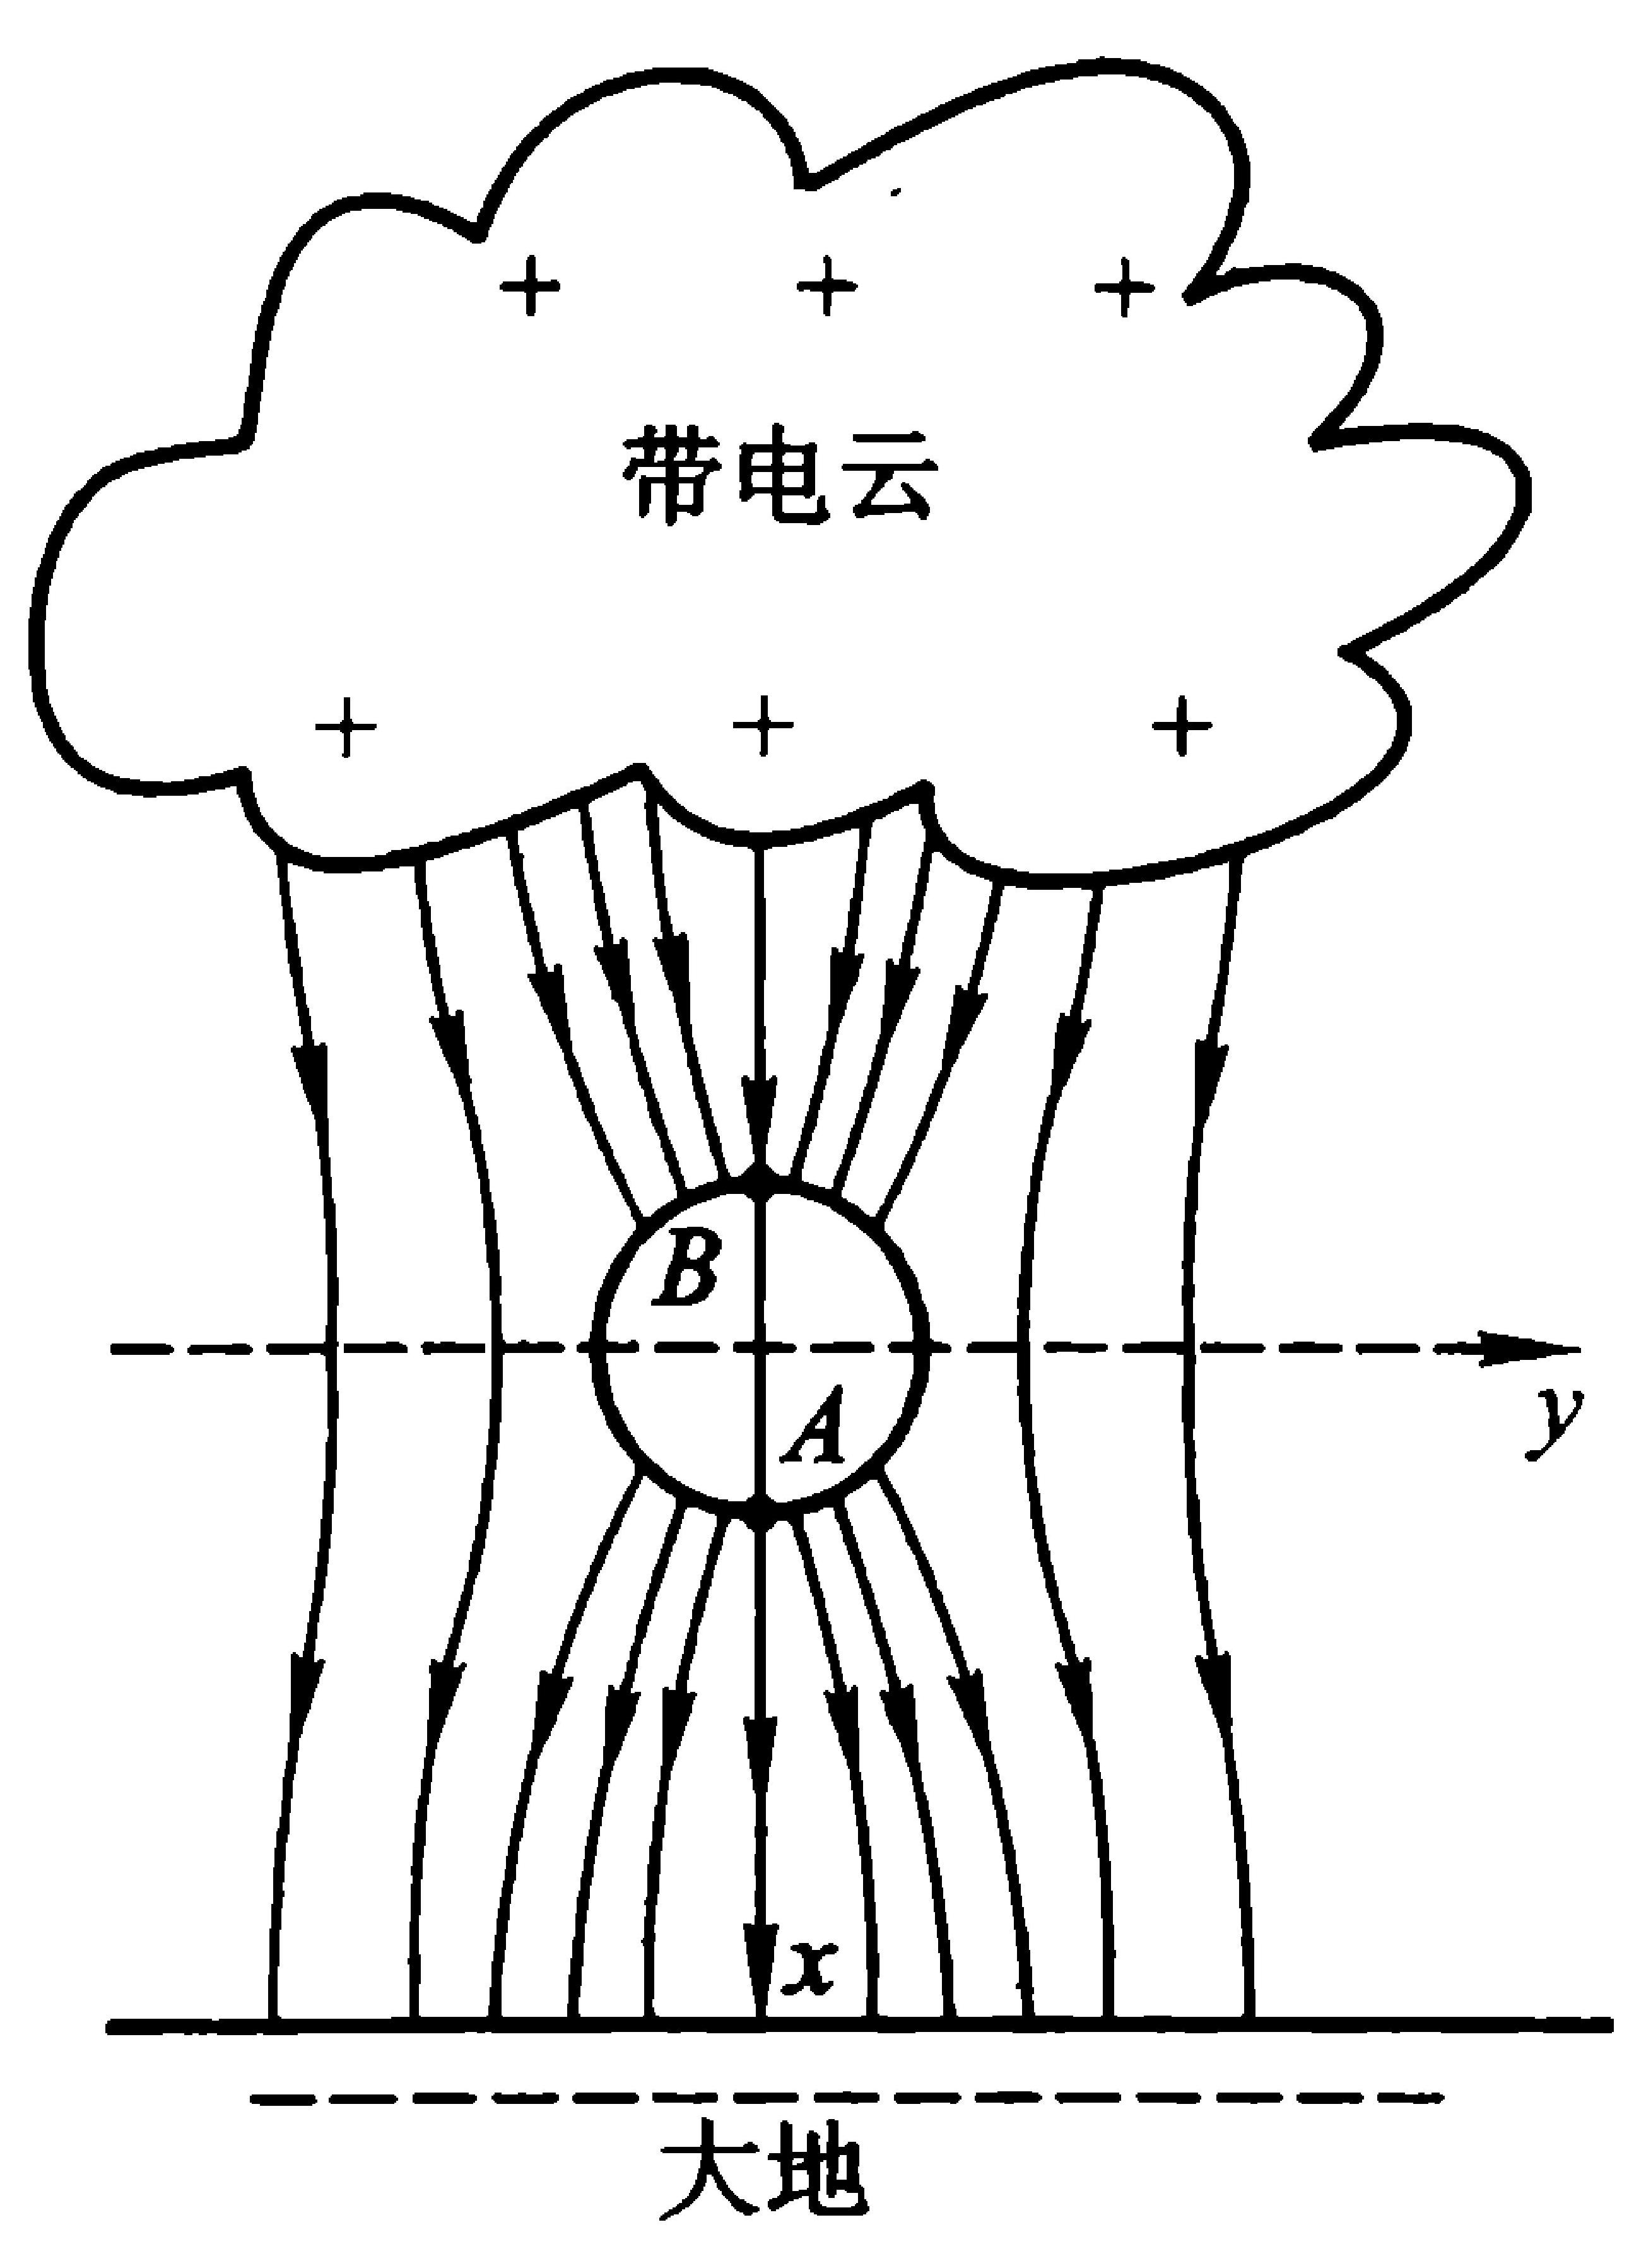
\includegraphics[width=0.3\textwidth]{wire.jpg}
    \end{center}
    \vspace{-20pt}
    \caption{输电线示意图.}
    \vspace{-10pt}
    \label{fig:wire}
  \end{wrapfigure}
首先需要把这个物理问题表为定解问题. 取圆柱的轴为 $z$ 轴. 
如果圆柱 “无限长”, 那么, 这个静电场的电场强度、电势显然跟 $z$ 无关, 我们只需在 $x y$ 平面上加以研究就够了.
图\ref{fig:wire}画的正是 $xy$ 平面上的静电场, 圆柱面在
$xy$ 平面的剖口是圆 $x^{2}+y^{2}=a^{2}$, 其中 $a$ 是圆柱的半径.

柱外的空间中没有电荷, 所以电势 $u$ 满足二维的拉普拉斯方程

$$
u_{x x}+u_{y y}=0 \quad \text { (柱外). }
$$

导体中的电荷既然不再移动, 这说明导体中各处电势相同. 又因为电势只具有相对的意义, 不妨把电势的零点取在导体上, 从而写出边界条件

$$
\left.u\right|_{x^{2}+y^{2}=a^{2}}=0 .
$$

按照分离变数法, 以 $u(x, y)=X(x) Y(y)$ 代入拉普拉斯方程固然不难把它分解为两个常微分方程,但代入上述边界条件却只能得到

$$
X(x) Y\left(\sqrt{a^{2}-x^{2}}\right)=0
$$
不能分解为 $X(x)$ 或 $Y(y)$ 的边界条件. 事实上, 既然边界是圆, 直角坐标系显然是不适当的, 必须采用平面极坐标系.

“柱外空间中的电势 $u$ 满足拉普拉斯方程” 就表为
\begin{equation}
    \frac{\partial^{2} u}{\partial \rho^{2}}+\frac{1}{\rho} \frac{\partial u}{\partial \rho}+
    \frac{1}{\rho^{2}} \frac{\partial^{2} u}{\partial \varphi^{2}}=0 \quad(\rho>a)
    \label{eq:laplace_2d}
\end{equation}
式中 $\rho$ 是极径, $\varphi$ 是极角. “导体电势为零” 就表为齐次的边界条件
\begin{equation}
    \left.u\right|_{\rho=a}=0 .
    \label{eq:laplace_2d_bc}
\end{equation}


在 “无限远” 处的静电场仍然保持为匀强的 $\bE_{0}$. 由于选取了 $x$ 轴平行于 
$\bE_{0}$, 所以在无限远处, $E_{y}=0, E_{x}=E_{0}$, 即 $-\partial u / \partial x=E_{0}$, 
亦即 $u=-E_{0} x=$ $-E_{0} \rho \cos \varphi$. 另外, 导体圆柱还可能带电, 
若单位长度导体带的电量为 $q_{0}$, 它在圆柱外产生的电势为 $\left(q_{0} / 2 \pi \varepsilon_{0}\right) \ln (1 / \rho)$, 
因而还有一个非齐次的边界条件

\begin{equation}
    \left.u\right|_{\rho \rightarrow \infty} \sim u_{0}+
    \frac{q_{0}}{2 \pi \varepsilon_{0}} \ln \frac{1}{\rho}-E_{0} \rho \cos \varphi
    \label{eq:u_rho_infty}
\end{equation}
其中 $u_{0}$ 为常数, 其数值跟电势的零点选取有关. 这里要求其满足在圆柱导体侧面上电势为零. 
问题归结为求解平面极坐标系定解问题 \eqref{eq:laplace_2d}, \eqref{eq:laplace_2d_bc}.

按照前面的步骤, 以分离变数形式的试探解
$$
u(\rho, \varphi)=R(\rho) \Phi\left(\varphi\right)
$$
代入拉普拉斯方程\eqref{eq:laplace_2d}, 得
$$
\frac{\rho}{R} \cdot \frac{d}{d \rho}\left(\rho \frac{d R}{d \rho}\right)=-\frac{\Phi^{\prime \prime}}{\Phi}
$$

上式左边是 $\rho$ 的函数,与 $\varphi$ 无关; 右边是 $\varphi$ 的函数,与 $\rho$ 无关.
 两边不可能相等, 除非两边实际上是同一个常数. 把这常数记作 $\lambda$,

$$
-\frac{\Phi^{\prime \prime}}{\Phi}=\lambda=\frac{\rho}{R} \cdot \frac{d}{d \rho}\left(\rho \frac{d R}{d \rho}\right)
$$

这就分解为两个常微分方程

\begin{eqnarray}
        \Phi^{\prime \prime}+\lambda \Phi &=& 0, \\
        \label{eq:Phi}
        \rho^{2} R^{\prime \prime}+\rho R^{'}-\lambda R  &=& 0.
        \label{eq:R}
\end{eqnarray}
常微分方程\eqref{eq:Phi}隐含着一个附加条件. 
事实上, 一个确定地点的极角可以加减 $2 \pi$ 的整倍数, 而电势 $u$ 在确定的地点应具确定数值, 
所以 $u(\rho, \varphi$ $+2 \pi)=u(\rho, \varphi)$ , 
即 $R(\rho) \Phi(\varphi+2 \pi)=R(\rho) \Phi(\varphi)$ ,亦即
\begin{equation}
    \Phi(\varphi+2 \pi)=\Phi(\varphi)
    \label{eq:Phi_bc}
\end{equation}
这叫做自然的周期条件. 常微分方程\eqref{eq:Phi} 与条件\eqref{eq:Phi_bc} 构成本征值问题. 
同样取 $\lambda$ 为实数, 不难求得方程的解为
\begin{equation}
\Phi(\varphi)= 
    \begin{cases}
        A \cos \sqrt{\lambda} \varphi+B \sin \sqrt{\lambda} \varphi & (\lambda>0), 
        \\ 
        A+B \varphi & (\lambda=0), 
        \\ 
        A e^{\sqrt{-\lambda \varphi}}+B e^{-\sqrt{-\lambda \varphi}} & (\lambda<0) .
    \end{cases}
\end{equation}

从而, 求得本征值
\begin{equation}
    \lambda =m^{2} \quad(m=0,1,2, \cdots) ; \\
    \label{eq:Phi_ev}
\end{equation}
和本征函数
\begin{equation}
\Phi(\varphi) = \begin{cases}A \cos m \varphi+B \sin m \varphi & (m \neq 0), \\
A & (m=0)\end{cases}
\label{eq:Phi_ef}
\end{equation}
以本征值\eqref{eq:Phi_ev}代入常微分方程\eqref{eq:R},
$$
\rho^{2} \frac{d^{2} R}{d \rho^{2}}+\rho \frac{d R}{d \rho}-m^{2} R=0
$$

这是欧拉型常微分方程, 作代换 $\rho=e^{t}$, 即 $t=\ln \rho$, 方程化为
$$
\frac{d^{2} R}{d t^{2}}-m^{2} R=0
$$
其解为

$$
R(\rho)= \begin{cases}C e^{m t}+D e^{-m t}=C \rho^{m}+D \frac{1}{\rho^{m}} & (m \neq 0) \\ C+D t=C+D \ln \rho & (m=0)\end{cases}
$$

这样, 分离变数形式的本征解是

$$
\begin{gathered}
u_{0}(\rho, \varphi)=C_{0}+D_{0} \ln \rho \\
u_{m}(\rho, \varphi)=\rho^{m}\left(A_{m} \cos m \varphi+B_{m} \sin m \varphi\right)+\rho^{-m}\left(C_{m} \cos m \varphi+D_{m} \sin m \varphi\right)
\end{gathered}
$$

拉普拉斯方程是线性的, 它的一般解应是所有本征解的叠加, 即

\begin{equation}
\begin{aligned}
u(\rho, \varphi)= & C_{0}+D_{0} \ln \rho+\sum_{m=1}^{\infty} \rho^{m}\left(A_{m} \cos m \varphi+B_{m} \sin m \varphi\right) \\
& +\sum_{m=1}^{\infty} \rho^{-m}\left(C_{m} \cos m \varphi+D_{m} \sin m \varphi\right)
\end{aligned}
\label{eq:u_rho_phi_general}
\end{equation}

为确定\eqref{eq:u_rho_phi_general} 中的系数, 把它代入边界条件. 先代入齐次边界条件\eqref{eq:laplace_2d_bc},
$$
\begin{gathered}
C_{0}+D_{0} \ln a+\sum_{m=1}^{\infty} a^{m}\left(A_{m} \cos m \varphi+B_{m} \sin m \varphi\right) \\
+\sum_{m=1}^{\infty} a^{-m}\left(C_{m} \cos m \varphi+D_{m} \sin m \varphi\right)=0
\end{gathered}
$$
一个傅里叶级数等于零, 意味着所有傅里叶系数为零, 即
$$
C_{0}+D_{0} \ln a=0, \quad a^{m} A_{m}+a^{-m} C_{m}=0, \quad a^{m} B_{m}+a^{-m} D_{m}=0
$$
由此,

$$
C_{0}=-D_{0} \ln a, \quad C_{m}=-A_{m} a^{2 m}, \quad D_{m}=-B_{m} a^{2 m}
$$

以此代入\eqref{eq:u_rho_phi_general}, 得
\begin{equation}
    \begin{aligned}
        u(\rho, \varphi)= & D_{0} \ln \frac{\rho}{a}+\sum_{m=1}^{\infty} \rho^{m}\left(A_{m} \cos m \varphi+B_{m} \sin m \varphi\right) \\
        & +\sum_{m=1}^{\infty} \rho^{-m}\left(-a^{2 m} A_{m} \cos m \varphi-a^{2 m} B_{m} \sin m \varphi\right)
        \end{aligned}
        \label{eq:u_rho_phi_2}
\end{equation}


将 \eqref{eq:u_rho_phi_2} 代入非齐次的边界条件\eqref{eq:u_rho_infty}, 在 $\rho$ 很大的地方, 有
\begin{equation}
    \begin{gathered}
        D_{0} \ln \frac{\rho}{a}+\sum_{m=1}^{\infty}\left[A_{m}\left(\rho^{m}-\frac{a^{2 m}}{\rho^{m}}\right) \cos m \varphi+B_{m}\left(\rho^{m}-\frac{a^{2 m}}{\rho^{m}}\right) \sin m \varphi\right] \\
        \sim u_{0}+\frac{q_{0}}{2 \pi \varepsilon_{0}} \ln \frac{1}{\rho}-E_{0} \rho \cos \varphi
    \end{gathered}
    \label{eq:matching}
\end{equation}
既然主要部分是 $\rho^{1}$ 项, 可见上式中不应出现 $\rho^{m}(m>1)$ 的项 (否则 $\rho^{m}$ 项就成了主要部分)。这是说,
$$
A_{m}=0, B_{m}=0 . \quad(m>1)
$$

从\eqref{eq:matching}比较系数, 还能知道
$$
B_{1}=0, A_{1}=-E_{0}, D_{0}=-\frac{q_{0}}{2 \pi \varepsilon_{0}}, 
u_{0}=-D_{0} \ln a=\frac{q_{0}}{2 \pi \varepsilon_{0}} \ln a
$$
最后得柱外的静电势为

$$
u(\rho, \varphi)=\frac{q_{0}}{2 \pi \varepsilon_{0}} \ln \frac{a}{\rho}-E_{0} \rho \cos \varphi+E_{0} \frac{\dot{a}^{2}}{\rho} \cos \varphi
$$

简单谈谈所得解答的物理含义. 
第一项是圆柱导体原来所带电荷在导体周围产生的电势. 
由于 $\rho>a$, 就好像是位于轴线 $\rho=0$ 上的带电导线产生的电势. 
常数 $u_{0}$ 的数值保证在圆柱导体的侧面上电势为零. 中间项正是原来的匀强静电场中的电势分布. 
最后一项, 即 $E_{0}\left(a^{2} / \rho\right) \cos \varphi$ 对于大的 $\rho$ 可以忽略,
所以它代表在圆柱邻近对匀强电场的修正, 这自然是柱面在匀强电场中产生的感应电荷形成的电势. 圆柱导体外的电场线分布见图 8-3a.

设圆柱体原来并不带电, 从而 $D_{0}=0$, 这时只含两项,

$$
u(\rho, \varphi)=-E_{0} \rho \cos \varphi+E_{0} \frac{a^{2}}{\rho} \cos \varphi
$$
$A$ 点和 $B$ 点的电场强度是
$$
E=-\left.\frac{\partial u}{\partial \rho}\right|_{\substack{\rho=a \\ \varphi=0, \pi}}
=\left.\left(E_{0} \cos \varphi+E_{0} \frac{a_{2}}{\rho} \cos \varphi\right)\right|_{\substack{\rho=a \\ \varphi=0, \pi}}
= \pm 2 E_{0}
$$
是原来的匀强电场的两倍! 所以在这两处特别容易击穿. 而且不管圆柱的半径多么小, 这个结论总是对的!

在$y$ 轴上的电势是
$$
u_{\varphi= \pm \pi / 2}=\left.\left(-E_{0} \rho \cos \varphi+E_{0} \frac{a_{2}}{\rho} \cos \varphi\right)\right|_{\varphi= \pm \pi / 2}=0
$$
跟导体圆柱的电势相同. 

非齐次方程齐次边界条件参考教材中的傅里叶级数法和冲量定理法. 非齐次边界条件的处理不做要求.


\section{非齐次方程齐次边界条件}

% 上一节研究了齐次方程的定解问题. 本节要研究非齐次振动方程和输运方程的定解问题.

% 我们仍然限于齐次的边界条件, 关于非齐次边界条件的处理请看下一节.

本节先介绍傅里叶级数法, 它直接求解非齐次方程的定解问题. 
接着是冲量定理法, 它把非齐次方程的定解问题转化为齐次方程的定解问题然后求解.

\subsection{(一) 傅里叶级数法}
$\S 8.1$ 中求解两端固定的弦的齐次振动方程定解问题, 得到的解 (8.1.14)具有傅里叶正弦级数的形式, 而且其系数 $A_{n}$ 和 $B_{n}$ 决定于初始条件 $\varphi(x)$ 和 $\psi(x)$ 的傅里叶正弦级数 (8.1.15). 至于采取正弦级数而不是一般的傅里叶级数的形式,则完全是由于两端都是第一类齐次边界条件 $\left.u\right|_{x=0}=0$ 和 $\left.u\right|_{x=l}=0$的原因.

分离变数法得出的这些结果给出提示: 不妨把所求的解本身展开为傅里叶级数, 即

$$
u(x, t)=\sum_{n} T_{n}(t) X_{n}(x)
$$

傅里叶级数 (8.2.1) 的基本函数族 $X_{n}(x)$ 为该定解问题齐次方程在所给齐次边界条件下的本征函数.

由于解是自变数 $x$ 和 $t$ 的函数, 因而 $u(x, t)$ 的傅里叶系数不是常数, 而是时间 $t$ 的函数, 把它记作 $T_{n}(t)$. 将待定解 (8.2.1) 代入泛定方程, 尝试分离出 $T_{n}(t)$ 的常微分方程, 然后求解.

例 1 求解定解问题

$$
\begin{gathered}
u_{t t}-a^{2} u_{x x}=A \cos \frac{\pi x}{l} \sin \omega t ; \\
\left.u_{x}\right|_{x=0}=0,\left.u_{x}\right|_{x=l}=0 ; \\
\left.u\right|_{t=0}=\varphi(x),\left.u_{t}\right|_{t=0}=\psi(x),(0<x<l) .
\end{gathered}
$$

解 级数展开的基本函数应是相应的齐次泛定方程 $u_{t u}-a^{2} u_{x x}=0$ 在所给齐次边界条件 $\left.u_{x}\right|_{x=0}=0$ 和 $\left.u_{x}\right|_{x=l}=0$ 下的本征函数. 我们已经熟悉这些本征函数, 它们是 $\cos \frac{n \pi x}{l}(n=0,1,2, \cdots)$. 这样, 试把所求的解展开为傅里叶余弦级数

$$
u(x, t)=\sum_{n=0}^{\infty} T_{n}(t) \cos \frac{n \pi x}{l}
$$

为了求解 $T_{n}(t)$ ,尝试把这个级数代入非齐次泛定方程 (8.2.2),

$$
\sum_{n=0}^{\infty}\left[T_{n}^{\prime \prime}+\frac{n^{2} \pi^{2} a^{2}}{l^{2}} T_{n}\right] \cos \frac{n \pi x}{l}=A \cos \frac{\pi x}{l} \sin \omega t
$$

等式左边是傅里叶余弦级数, 这提示我们把等式右边也展开为傅里叶余弦级数. 其实, 右边已经是傅里叶余弦级数, 它只有一个单项即 $n=1$ 的项. 于是, 比较两边的系数, 分离出 $T_{n}(t)$ 的常微分方程

$$
T_{1}^{\prime \prime}+\frac{\pi^{2} a^{2}}{l^{2}} T_{1}=A \sin \omega t, \quad T_{n}^{\prime \prime}+\frac{n^{2} \pi^{2} a^{2}}{l^{2}} T_{n}=0, \quad n \neq 1
$$

又把 $u(x, t)$ 的傅里叶余弦级数代入初始条件, 得

$$
\begin{aligned}
& \sum_{n=0}^{\infty} T_{n}(0) \cos \frac{n \pi}{l} x=\varphi(x)=\sum_{n=0}^{\infty} \varphi_{n} \cos \frac{n \pi}{l} x \\
& \sum_{n=0}^{\infty} T_{n}^{\prime}(0) \cos \frac{n \pi}{l} x=\psi(x)=\sum_{n=0}^{\infty} \psi_{n} \cos \frac{n \pi}{l} x .
\end{aligned}
$$

其中 $\varphi_{n} 、 \psi_{n}$ 分别为 $\varphi(x)$ 和 $\psi(x)$ 的傅里叶余弦级数 [ 以 $\cos (n \pi x / l)$ 为基本函数族] 的第 $n$ 个傅里叶系数. 等式 (8.2.5)、(8.2.6) 两边都是傅里叶余弦级数. 由于基本函数族 $\cos (n \pi x / l)$ 的正交性,等式两边对应同一基本函数的傅里叶系数必然相等; 于是得 $T_{n}(t)$ 的非零值初始条件

$$
\begin{aligned}
& \left\{\begin{array}{l}
T_{0}(0)=\varphi_{0}=\frac{1}{l} \int_{0}^{l} \varphi(\xi) d \xi, \\
T_{0}^{\prime}(0)=\psi_{0}=\frac{1}{l} \int_{0}^{l} \psi(\xi) d \xi ;
\end{array}\right. \\
& \left\{\begin{array}{l}
T_{n}(0)=\varphi_{n}=\frac{2}{l} \int_{0}^{l} \varphi(\xi) \cos \frac{n \pi \xi}{l} d \xi, \\
T_{n}^{\prime}(0)=\psi_{n}=\frac{2}{l} \int_{0}^{l} \psi(\xi) \cos \frac{n \pi \xi}{l} d \xi,
\end{array}\right.
\end{aligned}
$$

$T_{n}(t)$ 的常微分方程在初始条件 (8.2.7) 下的解是

$$
\begin{aligned}
& T_{0}(t)=\varphi_{0}+\psi_{0} t \\
& T_{1}(t)=\frac{A l}{\pi a} \frac{1}{\omega^{2}-\pi^{2} a^{2} / l^{2}}\left(\omega \sin \frac{\pi a t}{l}-\frac{\pi a}{l} \sin \omega t\right) \\
&+\varphi_{1} \cos \frac{\pi a t}{l}+\frac{l}{\pi a} \psi_{1} \sin \frac{\pi a t}{l}, \\
& T_{n}(t)=\varphi_{n} \cos ^{*} \frac{n \pi a t}{l}+\frac{l}{n \pi a} \psi_{n} \sin \frac{n \pi a t}{l} \quad(n \neq 0,1)
\end{aligned}
$$

(8.2.9) 的第一项为 $T_{1}(t)$ 的非齐次常微分方程的特解, 满足零值初始条件. (8.2.9) 的后两项之和及 $(8.2 .10)$ 分别为 $T_{1}(t)$ 和 $T_{n}(t)(n \neq 0,1)$ 的齐次
常微分方程的解, 满足非零值初始条件 (8.2.7).

这样, 所求的解是

$$
\begin{aligned}
u(x, t)= & \frac{A l}{\pi a} \cdot \frac{1}{\omega^{2}-\pi^{2} a^{2} / l^{2}}\left(\omega \sin \frac{\pi a t}{l}-\frac{\pi a}{l} \sin \omega t\right) \cos \frac{\pi x}{l}+\varphi_{0}+ \\
& \psi_{0} t+\sum_{n=1}^{\infty}\left(\varphi_{n} \cos \frac{n \pi a t}{l}+\frac{l}{n \pi a} \psi_{n} \sin \frac{n \pi a t}{l}\right) \cos \frac{n \pi x}{l}
\end{aligned}
$$

尝试成功了, 这个方法叫做傅里叶级数法. 很明显, 这个方法的关键在于分离出 $T_{n}(t)$ 的常微分方程, 其中不可混杂着另一自变数 $x$, 这是怎样做到的呢? 原来, 这个级数展开的基本函数 $\cos (n \pi x / l)$ 正是相应齐次方程、齐次边界条件下用分离变数法求得的本征函数, 这才得以分离出 $T_{n}(t)$ 的常微分方程. 因此, 傅里叶级数法一定要与分离变数法相结合才能应用.

齐次振动方程和齐次输运方程问题当然也可以用傅里叶级数法 (结合分离变数法) 求解, 这时得到的 $T_{n}(t)$ 的常微分方程为齐次方程, 求解更容易. 建议读者用这样的方法重新求解上节的定解问题 (8.1.1) (8.1.3) 以及例 1 和例 2 , 这里就不赘述了.

综上所述, 可以看出, 对于振动和输运问题, 不论齐次还是非齐次方程定解问题, 傅里叶级数法结合分离变数法均可应用. 如仅用分离变数法, 则只能用于齐次方程齐次边界条件定解问题.

\subsection{(二) 冲量定理法}
求解非齐次振动方程和输运方程定解问题还可用冲量定理法. 这里仍然考虑边界条件是齐次的. 应用冲量定理法有一个前提, 即初始条件均取零值. 这其实无损于一般性. 现以两端固定弦的受迫振动为例, 如果初始条件是非零值, 则定解问题为

$$
\begin{aligned}
& u_{t t}-a^{2} u_{x x}=f(x, t) \\
& \left.u\right|_{x=0}=0,\left.u\right|_{x=l}=0 \\
& \left.u\right|_{t=0}=\varphi(x),\left.u_{t}\right|_{t=0}=\psi(x)
\end{aligned}
$$

由于泛定方程和定解条件都是线性的, 可以利用叠加原理, 把 $u$ 分解为 $u^{\mathrm{I}}$ 与 $u^{\mathrm{I}}$ 之和, 即

$$
u(x, t)=u^{\mathrm{I}}(x, t)+u^{\mathrm{I}}(x, t)
$$

并令 $u^{\mathrm{I}} 、 u^{\mathbb{1}}$ 分别满足

$$
\begin{array}{l|l}
u_{t t}^{\mathrm{I}}-a^{2} u_{x x}^{\mathrm{I}}=0, & u_{t t}^{\mathrm{II}}-a^{2} u_{x x}^{\mathrm{I}}=f(x, t), \\
\left.u^{\mathrm{I}}\right|_{x=0}=0,\left.u^{\mathrm{I}}\right|_{x=l}=0, & \left.u^{\mathrm{I}}\right|_{x=0}=0,\left.u^{\mathrm{II}}\right|_{x=l}=0, \\
\left.u^{\mathrm{I}}\right|_{t=0}=\varphi(x),\left.u_{t}^{\mathrm{I}}\right|_{t=0}=\psi(x) . & \left.u^{\mathrm{I}}\right|_{t=0}=0,\left.u_{t}^{\mathbb{I}}\right|_{t=0}=0
\end{array}
$$

把竖线两边对应的式子相叠加, 正好是原来的定解问题. 这样, 问题转化
为求解 $u^{\mathrm{I}}$ 和 $u^{\mathrm{I}} . u^{\mathrm{I}}$ 的初始条件是非零值, 但方程是齐次的, 可用上节方法求解; $u^{\text {II }}$ 的方程是非齐次的, 但初始条件已化为零值, 符合冲量定理法所提出的要求.

现在用冲量定理法来研究弦的非齐次振动方程定解问题

$$
\begin{gathered}
u_{u}-a^{2} u_{x x}=f(x, t) \\
\left.u\right|_{x=0}=0,\left.u\right|_{x=l}=0 \\
\left.u\right|_{t=0}=0,\left.\quad u_{t}\right|_{t=0}=0
\end{gathered}
$$

冲量定量法的物理思想
首先, 在物理上, 非齐次泛定方程 (8.2.12) 表明, 作用在每单位长弦上的外力 $F(x, t)=\rho f(x, t)$. 它从时刻零持续作用到时刻 $t$, 我们求解的是 $F(x$, $t$ )作用下, 在时刻 $t$ 的各处位移 $u(x, t)$.

冲量定理法的基本物理思想是把持续作用力看成许许多多前后相继的 “瞬时” 力, 把持续作用力引起的振动看作所有 “瞬时” 力引起的振动的叠加. 根据 (5.3.9), 持续作用的力 $F(x, t)$ 可以表示成

$$
\begin{aligned}
F(x, t) & =\int_{0}^{t} F(x, \tau) \delta(t-\tau) d \tau=\rho f(x, t) \\
& =\int_{0}^{t} \rho f(x, \tau) \delta(t-\tau) d \tau,
\end{aligned}
$$

其中 $F(x, \tau) \delta(t-\tau) d \tau$ 为作用在很短的时间区间 $(\tau, \tau+d \tau)$ 上而冲量为 $F(x, \tau) d \tau$ 的 “瞬时” 力. 把该瞬时力引起的振动记为 $u^{(\tau)}(x, t)$, 则 $u^{(\tau)}(x, t)$的定解问题为

$$
\begin{gathered}
u_{t u}^{(\tau)}-a^{2} u_{x x}^{(\tau)}=\frac{F(x, \tau)}{\rho} \delta(t-\tau) d \tau=f(x, \tau) \delta(t-\tau) d \tau \\
\left.u^{(\tau)}\right|_{x=0}=0,\left.u^{(\tau)}\right|_{x=l}=0, \\
\left.u^{(\tau)}\right|_{t=0}=0,\left.u_{t}^{(\tau)}\right|_{t=0}=0
\end{gathered}
$$

由于瞬时力 $F(x, \tau) \delta(t-\tau) d \tau$ 作用在时间区间 $(\tau, \tau+d \tau)$ 上, 从时刻零直到时刻 $\tau-0$, 它尚未起作用, 弦仍然是静止的, $\left.u^{(\tau)}\right|_{t=\tau-0}=0,\left.u_{t}^{(\tau)}\right|_{t=\tau-0}=$ 0 . 时刻 $\tau$, 该瞬时力开始作用, 至时刻 $\tau+d \tau$ 结束. 由于 $d \tau$ 很短, 弦上各质点 “来不及” 位移, 故在时刻 $\tau+d \tau$, 位移 $\left.u^{(\tau)}\right|_{t=\tau+d \tau}=0$. 再看时刻 $\tau+d \tau$的速度 $u_{t}^{(\tau)}$, 根据冲量定理, 从 $\tau-0$ 时刻到 $\tau+d \tau$ 时刻, 单位长度弦的动量变化等于瞬时力 $F(x, \tau) \delta(t-\tau) d \tau$ 的冲量, 故有

$$
\left.\rho u_{t}^{(\tau)}\right|_{t=\tau+d \tau}-\left.\rho u_{t}^{(\tau)}\right|_{t=\tau-0}=F(x, \tau) d \tau=\rho f(x, \tau) d \tau
$$

从而得到

$$
\left.u_{t}^{(\tau)}\right|_{t=\tau+d \tau}=f(x, \tau) d \tau
$$

如果改取 $\tau+d \tau$ 时刻作为初始时刻, 考察瞬时力 $F(x, \tau) \delta(t-\tau) d \tau$ 在 $\tau+$
$d \tau$ 时刻以后引起的振动 $u^{(\tau)}(x, t)$, 由于该瞬时力已经作用过了, 弦上不受外力, $u^{(r)}(x, t)$ 满足齐次方程, 其定解问题为

$$
\begin{gathered}
u_{t t}^{(\tau)}-a^{2} u_{x x}^{(\tau)}=0, \\
\left.u^{(\tau)}\right|_{x=0}=0,\left.u^{(\tau)}\right|_{x=l}=0, \\
\left.u^{(\tau)}\right|_{t=\tau+d \tau}=0,\left.u_{t}^{(\tau)}\right|_{t=\tau+d \tau}=f(x, \tau) d \tau .
\end{gathered}
$$

定解问题 (8.2.19) (8.2.20) 与定解问题 (8.2.16) (8.2.18) 是等价的. 从 (8.2.20) 可以看出 $u^{(\tau)}$ 必含有因子 $d \tau$, 若记 $u^{(\tau)}(x, t)=v(x, t ; \tau) d \tau$,则 $v(x, t ; \tau)$ 满足定解问题

$$
\begin{aligned}
& v_{t t}-a^{2} v_{x x}=f(x, \tau) \delta(t-\tau), \\
&\left.v\right|_{x=0}=0,\left.v\right|_{x=l}=0, \\
&\left.v\right|_{t=0}=0,\left.\quad v_{t}\right|_{t=0}=0 .
\end{aligned}
$$

即

$$
\begin{gathered}
v_{t t}-a^{2} v_{x x}=0, \\
\left.v\right|_{x=0}=0,\left.v\right|_{x=\imath}=0, \\
\left.v\right|_{t=\tau}=0,\left.\quad v_{t}\right|_{t=\tau}=f(x, \tau) .
\end{gathered}
$$

由于 $d \tau$ 很短, 在 (8.2.25) 中已将 $\tau+d \tau$ 时刻记为 $\tau$ 时刻, 定解问题 (8.2.24) (8.2.25) 为齐次方程问题, 可用前面的分离变数法或傅里叶级数法求解. 只是要注意, 前面两种方法中初始时刻为零时刻, 这里初始时刻为 $\tau$ 时刻, 因此前两种方法解中的 $t$ (表示距初始时刻零时刻的时间间隔), 在这里应换成 $t-\tau$.

定解问题 (8.2.12) (8.2.14) 是线性的, 适用叠加原理, 既然外加力是一系列瞬时力的叠加, 则定解问题 (8.2.12) (8.2.14) 的解也应是瞬时力所引起的振动的叠加. 计及所有瞬时力的影响, 就有

$$
u(x, t)=\sum_{\tau=0}^{t} u^{(\tau)}(x, t)=\int_{0}^{t} v(x, t ; \tau) d \tau
$$

$u(x, t)$ 就是定解问题 (8.2.12) (8.2.14) 的解. 这就从物理上给出了求解非齐次振动方程定解问题 (8.2.12) (8.2.14) 的方法, 因为利用了冲量定理,故称为冲量定理法.

回顾一下求解步骤, 为了求解非齐次振动方程定解问题 (8.2.12) (8.2.14), 把持续作用的力 $\rho f(x, t)$ 看作一系列前后相继的脉冲力 $\rho f(x, t)$ $\delta(t-\tau) d \tau$, 改为求解脉冲力 $\rho f(x, t) \delta(t-\tau) d \tau$ 从 $\tau$ 时刻起所引起的振动 $v(x$, $t ; \tau) d \tau, v(x, t ; \tau)$ 满足齐次振动方程定解问题 (8.2.24) (8.2.25), 解出 $v(x, t ; \tau)$ 后, 代入 $(8.2 .26)$, 对 $\tau$ 积分, 就能得到所求的解.

$u(x, t)$ 和 $u^{(\tau)}(x, t)$ 的量纲为 $[x], v(x, t ; \tau)$ 的量纲为 $[x] /[t]$. 只要注意 $\delta(t-\tau)$ 的量纲为 $1 /[t]$, 不难检验, 方程 (8.2.12) 和 (8.2.16) 中每一项的量纲均为 $[x] /[t]^{2}$, 而方程 (8.2.21) 中每一项的量纲同是 $[x] /[t]^{3}$. 因此, 从
量纲来分析, 方程 (8.2.12)、(8.2.16)、(8.2.19)、(8.2.21) 和 (8.2.24) 在物理上都是正确的, 这从另一个侧面, 证明冲量定理法在物理上是行得通的.

冲量定理法的数学验证

这里要验证, 由满足齐次振动方程定解问题 (8.2.24)、( 8.2 .22$)$ 、 (8. 2. 25) 的解 $v(x, t ; \tau)$ 通过积分 (8.2.26) 得到的 $u(x, t)$ 是非齐次振动方程定解问题 (8.2.12) (8.2.14) 的解.

首先验证边界条件. 由于 $\left.v\right|_{x=0}=0 ;\left.v\right|_{x=l}=0$, 因此,

$$
\left.u\right|_{x=0}=\left.\int_{0}^{t} v\right|_{x=0} d \tau=0,\left.u\right|_{x=l}=\left.\int_{0}^{t} v\right|_{x=l} d \tau=0
$$

$u(x, t)$ 满足齐次边界条件 (8.2.13).

其次验证初始条件. 由 (8.2.26) 知初始位移

$$
\left.u\right|_{t=0}=\left.\int_{0}^{0} v\right|_{t=0} d \tau=0
$$

为验证初始速度, 需利用积分号下求导的公式

$$
\begin{aligned}
\frac{d}{d t} \int_{\alpha(t)}^{\beta(t)} g(t ; \tau) d \tau= & \int_{\alpha(t)}^{\beta(t)} \frac{\partial g(t ; \tau)}{\partial t} d \tau+g[t ; \beta(t)] \frac{d \beta(t)}{d t} \\
& -g[t ; \alpha(t)] \frac{d \alpha(t)}{d t}
\end{aligned}
$$

这个公式在微积分教本中可以找到. 把这个公式应用于 (8.2.26), 有

$$
u_{t}(x, t)=\int_{0}^{t} v_{\iota}(x, t ; \tau) d \tau+v(x, t ; t)
$$

按 $(8.2 .25), v(x, \tau ; \tau)=0 \quad(0 \leqslant \tau \leqslant t)$. 所以,

$$
\begin{aligned}
& u_{t}(x, t)=\int_{0}^{t} v_{t}(x, t ; \tau) d \tau, \\
& \left.u_{t}\right|_{\imath=0}=\left.\int_{0}^{0} v_{t}\right|_{\imath=0} d \tau=0 .
\end{aligned}
$$

(8.2.14) 中的两个零值初始条件均成立.

最后验证非齐次方程. 对 (8.2.28) 应用求导公式(8.2.27),

$$
u_{t t}=\int_{0}^{t} \dot{v}_{t u}(x, t ; \tau) d \tau+v_{t}(x, t ; t)
$$

按 (8.2.25), $v_{t}(x, \tau ; \tau)=f(x, \tau)(0 \leqslant \tau \leqslant t)$. 所以,

$$
u_{t t}=\int_{0}^{t} v_{t t}(x, t ; \tau) d \tau+f(x, t)
$$

以(8.2.26) 和 (8.2.29) 代入非齐次方程 (8.2.12) 的左边, 则

$$
\begin{aligned}
u_{t u}-a^{2} u_{x x} & =\int_{0}^{t}\left(v_{t t}-a^{2} v_{x x}\right) d \tau+f(x, t)=\int_{0}^{t} 0 d \tau+f(x, t) \\
& =f(x, t)
\end{aligned}
$$

非齐次方程 (8.2.12) 得以满足, 其中利用了 $v$ 的齐次方程 (8.2.24).
数学验证全部完成, 冲量定理法在数学上成立. 这里还应指出一点: 边界条件 (8.2.13) 不必限于第一类齐次边界条件, 也可以是第二类或第三.类齐次边界条件, 甚至 $x=0$ 端与 $x=l$ 端的边界条件还可以是不同类的, 只要边界条件 (8.2.22) 的类型与 $(8.2 .13)$ 相同就行.

例 2 将例 1 中的初始条件改为零值, 用冲量定理法求解, 即求解定解问题

$$
\begin{aligned}
& u_{u}-a^{2} u_{x x}=A \cos \frac{\pi x}{l} \sin \omega t ; \\
& \left.u_{x}\right|_{x=0}=0,\left.\quad u_{x}\right|_{x=\imath}=0 ; \\
& \left.u\right|_{t=0}=0,\left.\quad u_{t}\right|_{t=0}=0
\end{aligned}
$$

解 应用冲量定理法, 先求解

$$
\begin{gathered}
v_{t}-a^{2} v_{x x}=0 ; \\
\left.v_{x}\right|_{x=0}=0,\left.\quad v_{x}\right|_{x=\imath}=0 ; \\
\left.v\right|_{\imath=\tau+0}=0,\left.\quad v_{\iota}\right|_{\imath=\tau+0}=A \cos \frac{\pi x}{l} \sin \omega \tau .
\end{gathered}
$$

参照边界条件, 试把解 $v$ 展开为傅里叶余弦级数

$$
v(x, t ; \tau)=\sum_{n=0}^{\infty} T_{n}(t, \tau) \cos \frac{n \pi x}{l}
$$

把这余弦级数代入泛定方程

$$
\sum_{n=0}^{\infty}\left[T_{n}^{\prime \prime}+\frac{n^{2} \pi^{2} a^{2}}{l^{2}} T_{n}\right] \cos \frac{n \pi x}{l}=0
$$

由此分离出 $T_{n}$ 的常微分方程

$$
T_{n}^{\prime \prime}+\frac{n^{2} \pi^{2} a^{2}}{l^{2}} T_{n}=0
$$

这个常微分方程的解是

$$
\begin{aligned}
& T_{0}(t ; \tau)=A_{0}(\tau) B_{0}(\tau)(t-\tau), \\
& T_{n}(t ; \tau)=A_{n}(\tau) \cos \frac{n \pi a(t-\tau)}{l}+B_{n}(\tau) \sin \frac{n \pi a(t-\tau)}{l} \quad(n=1,2, \cdots) .
\end{aligned}
$$

这样, 解 $v$ 具有傅里叶余弦级数形式, 为

$$
\begin{aligned}
v(x, t ; \tau)= & A_{0}(\tau)+B_{0}(\tau)(t-\tau) \\
& +\sum_{n=1}^{\infty}\left[A_{n}(\tau) \cos \frac{n \pi a(t-\tau)}{l}\right. \\
& \left.+B_{n}(\tau) \sin \frac{n \pi a(t-\tau)}{l}\right] \cos \frac{n \pi x}{l}
\end{aligned}
$$

至于系数 $A_{n}(\tau)$ 和 $B_{n}(\tau)$ 则由初始条件确定. 为此, 把上式代入初始条件,

$$
\begin{gathered}
A_{0}(\tau)+\sum_{n=1}^{\infty} A_{n}(\tau) \cos \frac{n \pi x}{l}=0 \\
B_{0}(\tau)+\sum_{n=1}^{\infty} B_{n}(\tau) \frac{n \pi a}{l} \cos \frac{n \pi x}{l}=A \cos \frac{\pi x}{l} \sin \omega \tau .
\end{gathered}
$$

右边的 $A \cos \frac{\pi x}{l} \sin \omega \tau$ 也是傅里叶余弦级数, 它只有一个单项即 $n=1$ 的项. 比较两边系数, 得

$$
A_{n}(\tau)=0, B_{1}(\tau)=A \frac{l}{\pi a} \sin \omega \tau, B_{n}(\tau)=0, \quad(n=2,3, \cdots)
$$

到此, 已求出 $v(x, t ; \tau)$,

$$
v(x, t ; \tau)=A \frac{l}{\pi a} \sin \omega \tau \sin \frac{\pi a(t-\tau)}{l} \cos \frac{\pi x}{l} .
$$

按照 (8.2.26), 得出答案

$$
\begin{aligned}
u(x, t) & =\int_{0}^{t} v(x, t ; \tau) \\
& =\frac{A l}{\pi a} \cos \frac{\pi x}{l} \int_{0}^{l} \sin \omega \tau \sin \frac{\pi a(t-\tau)}{l} d \tau \\
& =\frac{A l}{\pi a} \frac{1}{\omega^{2}-\pi^{2} a^{2} / l^{2}}\left(\omega \sin \frac{\pi a}{l} t-\frac{\pi a}{l} \sin \omega t\right) \cos \frac{\pi x}{l} .
\end{aligned}
$$

输运问题, 如泛定方程是非齐次的, 完全可以仿照冲量定理法加以处理.比如, 研究定解问题

$$
\begin{gathered}
u_{t}-a^{2} u_{x x}=f(x, t), \\
\left.u_{x}\right|_{x=0}=0,\left.u_{x}\right|_{x=l}=0, \\
\left.u\right|_{t=0}=0 .
\end{gathered}
$$

非齐次泛定方程 (8.2.30) 表明, 每单位长度上的热源强度为 $c \rho f(x, t)$. 这热源从时刻零一直延续到时刻 $t$, 现在求解的是热源强度 $c \rho f(x, t)$ 的影响下,在时刻 $t$ 的温度分布.

仿照冲量定理法对非齐次振动方程定解问题的处理,这里按照 (5.3.9),将持续作用的热源看作许许多多前后相继的 “瞬时” 热源 $c \rho f(x, t) \delta(t-\tau) d \tau$的叠加, “瞬时” 热源 $c \rho f(x, \tau) \delta(t-\tau) d \tau$ 作用于时间区间 $(\tau, \tau+d \tau)$, 提供的热量为 $c \rho f(x, \tau) d \tau$, 记它所产生的温度分布为 $v(x, t ; \tau) d \tau$, 类似地可导出 $v(x, t ; \tau)$ 的定解问题为

$$
\begin{gathered}
v_{t}-a^{2} v_{x x}=f(x, \tau) \delta(t-\tau) \\
\left.v_{x}\right|_{x=0}=0,\left.v_{x}\right|_{x=l}=0 \\
\left.v\right|_{t=0}=0
\end{gathered}
$$

直到 $\tau-0$ 时刻, 瞬时热源尚未起作用, 从初始条件 $\left.v\right|_{t=0}=0$ 得 $\left.v\right|_{t=\tau-0}$
$=0 . \tau$ 时刻, 瞬时热源 $c \rho f(x, \tau) \delta(t-\tau) d \tau$ 开始起作用, 至 $\tau+d \tau$ 时刻, 作用结束, 瞬时热源放出的热量, 使 $\tau+d \tau$ 时刻的温度增加到 $\left.v\right|_{t=\tau+d \tau}$, 于是

$$
c \rho\left(\left.v\right|_{t=\tau+d \tau}-\left.v\right|_{t=\tau-0}\right) d \tau=c \rho f(x, \tau) d \tau
$$

从而

$$
\left.v\right|_{t=\tau+d \tau}=f(x, \tau) .
$$

这是 $\tau+d \tau$ 时刻的温度分布, 如果把 $\tau+d \tau$ 时刻作为初始时刻, 研究瞬时热源在 $\tau+d \tau$ 时刻以后产生的温度分布 $v(x, t ; \tau) d \tau$ ,则 $v(x, t ; \tau)$ 的定解问题为

$$
\begin{gathered}
v_{t}-a^{2} v_{x x}=0, \\
\left.v_{x}\right|_{x=0}=0,\left.v_{x}\right|_{x=l}=0, \\
\left.v\right|_{t=\tau}=f(x, \tau) .
\end{gathered}
$$

因为瞬时热源已经作用过了, 故 (8.2.36) 为齐次方程. 由于 $d \tau$ 很短, (8.2.37) 中将初始时刻 $\tau+d \tau$ 记为 $\tau$ 时刻. 定解问题 (8.2.36)、(8.2.34)、 (8.2.37) 与定解问题 (8.2.33) (8.2.35) 等价, 已是齐次泛定方程、齐次边界条件, 可用分离变数法或傅里叶级数法求解, 不过要注意, 原来求解公式中的 $t$ 这里应换为 $t-\tau$.

定解问题 (8.2.30) (8.2.32) 是线性的, 叠加原理也适用. 考虑所有瞬时热源产生的影响, 把这些影响叠加起来, 就得到此定解问题的解 $u(x, t)$,于是有

$$
u(x, t)=\int_{0}^{t} v(x, t ; \tau) d \tau
$$

同样, 可从数学上验证这样得到的 $u(x, t)$ 确实满足定解问题 (8.2.30) (8.2.32), 请读者去完成, 这里不赘述了.
\section{非齐次边界条件的处理}
\label{eq:inhomo_boundary}

在 $\S 8.1$ 和 $\S 8.2$ 两节中, 不管是齐次还是非齐次振动方程和输运方程,它们的定解问题的解法都有一个前提:边界条件是齐次的.

但是, 在实际问题中, 常有非齐次边界条件出现, 那么, 这样的定解问题又如何求解呢? 由于定解问题是线性的,处理的原则是利用叠加原理,把非齐次边界条件问题转化为另一未知函数的齐次边界条件问题. 请看例题.

\subsection{(一) 一般处理方法}
例 1 自由振动问题

$$
\begin{gathered}
u_{t t}-a^{2} u_{x x}=0, \\
\left.u\right|_{x=0}=\mu(t),\left.u\right|_{x=l}=\nu(t), \\
\left.u\right|_{t=0}=\varphi(x),\left.u_{t}\right|_{t=0}=\psi(x) .
\end{gathered}
$$

边界条件 (8.3.2) 是非齐次的.
选取一个函数 $v(x, t)$, 使其满足非齐次边界条件 (8.3.2), 为了简单起见, 不妨取 $v(x, t)$ 为 $x$ 的线性函数, 即

$$
v(x, t)=A(t) x+B(t) \text {. }
$$

将 (8.3.4) 代入 (8.3.2), 解得

$$
v(x, t)=\frac{[\nu(t)-\mu(t)]}{l} x+\mu(t)
$$

利用叠加原理, 令

$$
u(x, t)=v(x, t)+w(x, t) .
$$

将 (8.3.5)、(8.3.6) 代入定解问题 (8.3.1) (8.3.3), 得 $w(x, t)$ 的定解问题

$$
\begin{gathered}
w_{t u}-a^{2} w_{\imath \imath}=-v_{\imath t}+a^{2} v_{x x}=\frac{x}{l}\left[\mu^{\prime \prime}(t)-\nu^{\prime \prime}(t)\right]-\mu^{\prime \prime}(t), \\
\left.w\right|_{x=0}=0,\left.w\right|_{x=l}=0, \\
\left.w\right|_{t=0}=\varphi(x)-\left.v\right|_{\imath=0}=\varphi(x)+\frac{1}{l}[\mu(0)-\nu(0)] x-\mu(0), \\
\left.w_{\imath}\right|_{\imath=0}=\psi(x)-\left.v_{t}\right|_{t=0}=\psi(x)+\frac{1}{l}\left[\mu^{\prime}(0)-\nu^{\prime}(0)\right] x-\mu^{\prime}(0) .
\end{gathered}
$$

虽然 $w(x, t)$ 的方程 (8.3.7)一般是非齐次的,但是,定解问题 (8.3.7) (8.3.9) 具有齐次边界条件, 可按 $\S 8.2$ 求解.

这里还要特别说一下 $x=0$ 和 $x=l$ 两端都是第二类非齐次边界条件 $\left.u_{x}\right|_{x=0}$ $=\mu(t),\left.u_{x}\right|_{x=l}=\nu(t)$ 的情况. 如果仍按 (8.3.4) 取 $x$ 的线性函数作为 $v$, 则代入非齐次边界条件得

$$
\left.v_{x}\right|_{x=0}=A(t)=\mu(t),\left.\quad v_{x}\right|_{x=l}=A(t)=\nu(t) .
$$

除非 $\mu(t)=\nu(t)$, 否则这两式互相矛盾. 这时不妨改试

$$
v(x, t)=A(t) x^{2}+B(t) x .
$$

\subsection{(二) 特殊处理方法}
例 2 弦的 $x=0$ 端固定, $x=l$ 端受迫作谐振动 $A \sin \omega t$, 弦的初始位移和初始速度都是零, 求弦的振动. 这个定解问题是

$$
\begin{gathered}
u_{t t}-a^{2} u_{x x}=0 \quad(x<0<l), \\
\left.u\right|_{x=0}=0,\left.\quad u\right|_{x=l}=A \sin \omega t, \\
\left.u\right|_{t=0}=0,\left.\quad u_{t}\right|_{t=0}=0 .
\end{gathered}
$$

$x=l$ 端为非齐次边界条件.

如果按上述一般处理方法, 应取 $v(x, t)=(A \sin \omega t / l) x$, 但是, 相应的 $w(x, t)$ 的定解问题中泛定方程为 $w_{u}-a^{2} w_{x x}=-\left(v_{u t}-a^{2} v_{x x}\right)=\left(A \omega^{2} x / l\right) \sin \omega t$,是非齐次方程, 求解麻烦. 能否有较为简便的方法呢?

由于求解的是弦在 $x=l$ 端受迫作谐振动 $A \sin \omega t$ 情况下的振动, 它一定有一个特解 $v(x, t)$, 满足齐次方程 (8.3.11)、非齐次边界条件 (8.3.12), 且跟 $x$
$=l$ 端同步振动, 即其时间部分的函数亦为 $\sin \omega t$, 就是说, 特解具有分离变数的形式:

$$
v(x, t)=X(x) \sin \omega t
$$

将(8.3.14) 代入 (8.3.11)、

$$
\begin{aligned}
& (8.3 .12), \text { 得 } \\
& \left\{\begin{array}{l}
X^{\prime \prime}+\left(\frac{\omega}{a}\right)^{2} X=0, \\
X(0)=0, X(l)=A .
\end{array}\right.
\end{aligned}
$$

将常微分方程 (8.3.15) 的解 $X(x)=C \cos (\omega x / a)+D \sin (\omega x / a)$ 代入 (8.3.16), 由此确定 $X(x)=[A / \sin (\omega l / a)] \sin (\omega x / a)$, 从而

$$
v(x, t)=\frac{A}{\sin \frac{\omega l}{a}} \sin \frac{\omega x}{a} \sin \omega t
$$

于是令

$$
u(x, t)=v(x, t)+w(x, t),
$$

将 (8.3.17)、(8.3.18) 代入 (8.3.11) (8.3.13), 得 $w(x, t)$ 的定解问题

$$
\begin{gathered}
w_{t t}-a^{2} w_{x x}=-\left(v_{x x}-a^{2} v_{x x}\right)=0 \\
\left.w\right|_{x=0}=0,\left.\quad w\right|_{x=\imath}=0 \\
\left.w\right|_{\imath=0}=0,\left.\quad w_{\imath}\right|_{t=0}=-A \omega \frac{\sin (\omega x / a)}{\sin (\omega l / a)}
\end{gathered}
$$

定解问题 (8.3.19) (8.3.21) 为齐次方程、齐次边界条件, 可用分离变数法求解, 其一般解由 (8.1.14) 给出, 因此,

$$
w(x, t)=\sum_{n=1}^{\infty}\left(A_{n} \cos \frac{n \pi a}{l} t+B_{n} \sin \frac{n \pi a}{l} t\right) \sin \frac{n \pi}{l} x
$$

其中系数 $A_{n}$ 和 $B_{n}$ 可由 (8.1.16) 确定, 得

$$
\begin{aligned}
A_{n} & =0 \\
B_{n} & =\frac{2}{n \pi a} \int_{0}^{l}(-A \omega) \frac{\sin (\omega \xi / a)}{\sin (\omega l / a)} \sin \frac{n \pi \xi}{l} d \xi \\
& =\frac{-2 A \omega}{n \pi a \sin (\omega l / a)}\left[-\frac{\sin (\omega / a+n \pi / l) \xi}{2(\omega / a+n \pi / l)}+\frac{\sin (\omega / a-n \pi / l) \xi}{2(\omega / a-n \pi / l)}\right]_{0}^{l} \\
& =\frac{A \omega}{n \pi a \sin (\omega l / a)}\left[\frac{\sin (\omega l / a+n \pi)}{\omega / a+n \pi / l}-\frac{\sin (\omega l / a-n \pi)}{\omega / a-n \pi / l}\right] \\
& =(-1)^{n} \frac{A \omega}{n \pi a}\left[\frac{1}{\omega / a+n \pi / l}-\frac{1}{\omega / a-n \pi / l}\right] \\
& =(-1)^{n} \frac{2 A \omega}{a l} \cdot \frac{1}{\omega^{2} / a^{2}-n^{2} \pi^{2} / l^{2}} .
\end{aligned}
$$

这样

$$
\begin{aligned}
w(x, t)= & \frac{2 A \omega}{a l} \sum_{n=1}^{\infty} \frac{1}{\omega^{2} / a^{2}-n^{2} \pi^{2} / l^{2}} \sin \frac{n \pi a t}{l} \sin \frac{n \pi x}{l}, \\
u(x, t)= & A \frac{\sin (\omega x / a)}{\sin (\omega l / a)} \sin \omega t \\
& +\frac{2 A \omega}{a l} \sum_{n=1}^{\infty} \frac{1}{\omega^{2} / a^{2}-n^{2} \pi^{2} / l^{2}} \sin \frac{n \pi a t}{l} \sin \frac{n \pi x}{l} .
\end{aligned}
$$